\documentclass[10pt,journal,compsoc]{IEEEtran}
%
% If IEEEtran.cls has not been installed into the LaTeX system files,
% manually specify the path to it like:
% \documentclass[10pt,journal,compsoc]{../sty/IEEEtran}

% Some very useful LaTeX packages include:
% (uncomment the ones you want to load)


% *** MISC UTILITY PACKAGES ***
%
%\usepackage{ifpdf}
% Heiko Oberdiek's ifpdf.sty is very useful if you need conditional
% compilation based on whether the output is pdf or dvi.
% usage:
% \ifpdf
%   % pdf code
% \else
%   % dvi code
% \fi
% The latest version of ifpdf.sty can be obtained from:
% http://www.ctan.org/pkg/ifpdf
% Also, note that IEEEtran.cls V1.7 and later provides a builtin
% \ifCLASSINFOpdf conditional that works the same way.
% When switching from latex to pdflatex and vice-versa, the compiler may
% have to be run twice to clear warning/error messages.



% *** CITATION PACKAGES ***
%
\ifCLASSOPTIONcompsoc
  % IEEE Computer Society needs nocompress option
  % requires cite.sty v4.0 or later (November 2003)
  \usepackage[nocompress]{cite}
\else
  % normal IEEE
  \usepackage{cite}
\fi
% cite.sty was written by Donald Arseneau
% V1.6 and later of IEEEtran pre-defines the format of the cite.sty package
% \cite{} output to follow that of the IEEE. Loading the cite package will
% result in citation numbers being automatically sorted and properly
% "compressed/ranged". e.g., [1], [9], [2], [7], [5], [6] without using
% cite.sty will become [1], [2], [5]--[7], [9] using cite.sty. cite.sty's
% \cite will automatically add leading space, if needed. Use cite.sty's
% noadjust option (cite.sty V3.8 and later) if you want to turn this off
% such as if a citation ever needs to be enclosed in parenthesis.
% cite.sty is already installed on most LaTeX systems. Be sure and use
% version 5.0 (2009-03-20) and later if using hyperref.sty.
% The latest version can be obtained at:
% http://www.ctan.org/pkg/cite
% The documentation is contained in the cite.sty file itself.
%
% Note that some packages require special options to format as the Computer
% Society requires. In particular, Computer Society  papers do not use
% compressed citation ranges as is done in typical IEEE papers
% (e.g., [1]-[4]). Instead, they list every citation separately in order
% (e.g., [1], [2], [3], [4]). To get the latter we need to load the cite
% package with the nocompress option which is supported by cite.sty v4.0
% and later. Note also the use of a CLASSOPTION conditional provided by
% IEEEtran.cls V1.7 and later.



% *** MATH PACKAGES ***
%
%\usepackage{amsmath}
% A popular package from the American Mathematical Society that provides
% many useful and powerful commands for dealing with mathematics.
%
% Note that the amsmath package sets \interdisplaylinepenalty to 10000
% thus preventing page breaks from occurring within multiline equations. Use:
%\interdisplaylinepenalty=2500
% after loading amsmath to restore such page breaks as IEEEtran.cls normally
% does. amsmath.sty is already installed on most LaTeX systems. The latest
% version and documentation can be obtained at:
% http://www.ctan.org/pkg/amsmath


% *** SPECIALIZED LIST PACKAGES ***
%
%\usepackage{algorithmic}
% algorithmic.sty was written by Peter Williams and Rogerio Brito.
% This package provides an algorithmic environment fo describing algorithms.
% You can use the algorithmic environment in-text or within a figure
% environment to provide for a floating algorithm. Do NOT use the algorithm
% floating environment provided by algorithm.sty (by the same authors) or
% algorithm2e.sty (by Christophe Fiorio) as the IEEE does not use dedicated
% algorithm float types and packages that provide these will not provide
% correct IEEE style captions. The latest version and documentation of
% algorithmic.sty can be obtained at:
% http://www.ctan.org/pkg/algorithms
% Also of interest may be the (relatively newer and more customizable)
% algorithmicx.sty package by Szasz Janos:
% http://www.ctan.org/pkg/algorithmicx



% *** ALIGNMENT PACKAGES ***
%
%\usepackage{array}
% Frank Mittelbach's and David Carlisle's array.sty patches and improves
% the standard LaTeX2e array and tabular environments to provide better
% appearance and additional user controls. As the default LaTeX2e table
% generation code is lacking to the point of almost being broken with
% respect to the quality of the end results, all users are strongly
% advised to use an enhanced (at the very least that provided by array.sty)
% set of table tools. array.sty is already installed on most systems. The
% latest version and documentation can be obtained at:
% http://www.ctan.org/pkg/array


% IEEEtran contains the IEEEeqnarray family of commands that can be used to
% generate multiline equations as well as matrices, tables, etc., of high
% quality.


% *** SUBFIGURE PACKAGES ***
%\ifCLASSOPTIONcompsoc
%  \usepackage[caption=false,font=footnotesize,labelfont=sf,textfont=sf]{subfig}
%\else
%  \usepackage[caption=false,font=footnotesize]{subfig}
%\fi
% subfig.sty, written by Steven Douglas Cochran, is the modern replacement
% for subfigure.sty, the latter of which is no longer maintained and is
% incompatible with some LaTeX packages including fixltx2e. However,
% subfig.sty requires and automatically loads Axel Sommerfeldt's caption.sty
% which will override IEEEtran.cls' handling of captions and this will result
% in non-IEEE style figure/table captions. To prevent this problem, be sure
% and invoke subfig.sty's "caption=false" package option (available since
% subfig.sty version 1.3, 2005/06/28) as this is will preserve IEEEtran.cls
% handling of captions.
% Note that the Computer Society format requires a sans serif font rather
% than the serif font used in traditional IEEE formatting and thus the need
% to invoke different subfig.sty package options depending on whether
% compsoc mode has been enabled.
%
% The latest version and documentation of subfig.sty can be obtained at:
% http://www.ctan.org/pkg/subfig


% *** FLOAT PACKAGES ***
%
%\usepackage{fixltx2e}
% fixltx2e, the successor to the earlier fix2col.sty, was written by
% Frank Mittelbach and David Carlisle. This package corrects a few problems
% in the LaTeX2e kernel, the most notable of which is that in current
% LaTeX2e releases, the ordering of single and double column floats is not
% guaranteed to be preserved. Thus, an unpatched LaTeX2e can allow a
% single column figure to be placed prior to an earlier double column
% figure.
% Be aware that LaTeX2e kernels dated 2015 and later have fixltx2e.sty's
% corrections already built into the system in which case a warning will
% be issued if an attempt is made to load fixltx2e.sty as it is no longer
% needed.
% The latest version and documentation can be found at:
% http://www.ctan.org/pkg/fixltx2e


%\usepackage{stfloats}
% stfloats.sty was written by Sigitas Tolusis. This package gives LaTeX2e
% the ability to do double column floats at the bottom of the page as well
% as the top. (e.g., "\begin{figure*}[!b]" is not normally possible in
% LaTeX2e). It also provides a command:
%\fnbelowfloat
% to enable the placement of footnotes below bottom floats (the standard
% LaTeX2e kernel puts them above bottom floats). This is an invasive package
% which rewrites many portions of the LaTeX2e float routines. It may not work
% with other packages that modify the LaTeX2e float routines. The latest
% version and documentation can be obtained at:
% http://www.ctan.org/pkg/stfloats
% Do not use the stfloats baselinefloat ability as the IEEE does not allow
% \baselineskip to stretch. Authors submitting work to the IEEE should note
% that the IEEE rarely uses double column equations and that authors should try
% to avoid such use. Do not be tempted to use the cuted.sty or midfloat.sty
% packages (also by Sigitas Tolusis) as the IEEE does not format its papers in
% such ways.
% Do not attempt to use stfloats with fixltx2e as they are incompatible.
% Instead, use Morten Hogholm'a dblfloatfix which combines the features
% of both fixltx2e and stfloats:
%
% \usepackage{dblfloatfix}
% The latest version can be found at:
% http://www.ctan.org/pkg/dblfloatfix


%\ifCLASSOPTIONcaptionsoff
%  \usepackage[nomarkers]{endfloat}
% \let\MYoriglatexcaption\caption
% \renewcommand{\caption}[2][\relax]{\MYoriglatexcaption[#2]{#2}}
%\fi
% endfloat.sty was written by James Darrell McCauley, Jeff Goldberg and 
% Axel Sommerfeldt. This package may be useful when used in conjunction with 
% IEEEtran.cls'  captionsoff option. Some IEEE journals/societies require that
% submissions have lists of figures/tables at the end of the paper and that
% figures/tables without any captions are placed on a page by themselves at
% the end of the document. If needed, the draftcls IEEEtran class option or
% \CLASSINPUTbaselinestretch interface can be used to increase the line
% spacing as well. Be sure and use the nomarkers option of endfloat to
% prevent endfloat from "marking" where the figures would have been placed
% in the text. The two hack lines of code above are a slight modification of
% that suggested by in the endfloat docs (section 8.4.1) to ensure that
% the full captions always appear in the list of figures/tables - even if
% the user used the short optional argument of \caption[]{}.
% IEEE papers do not typically make use of \caption[]'s optional argument,
% so this should not be an issue. A similar trick can be used to disable
% captions of packages such as subfig.sty that lack options to turn off
% the subcaptions:
% For subfig.sty:
% \let\MYorigsubfloat\subfloat
% \renewcommand{\subfloat}[2][\relax]{\MYorigsubfloat[]{#2}}
% However, the above trick will not work if both optional arguments of
% the \subfloat command are used. Furthermore, there needs to be a
% description of each subfigure *somewhere* and endfloat does not add
% subfigure captions to its list of figures. Thus, the best approach is to
% avoid the use of subfigure captions (many IEEE journals avoid them anyway)
% and instead reference/explain all the subfigures within the main caption.
% The latest version of endfloat.sty and its documentation can obtained at:
% http://www.ctan.org/pkg/endfloat
%
% The IEEEtran \ifCLASSOPTIONcaptionsoff conditional can also be used
% later in the document, say, to conditionally put the References on a 
% page by themselves.


% *** PDF, URL AND HYPERLINK PACKAGES ***
%
%\usepackage{url}
% url.sty was written by Donald Arseneau. It provides better support for
% handling and breaking URLs. url.sty is already installed on most LaTeX
% systems. The latest version and documentation can be obtained at:
% http://www.ctan.org/pkg/url
% Basically, \url{my_url_here}.


% *** Do not adjust lengths that control margins, column widths, etc. ***
% *** Do not use packages that alter fonts (such as pslatex).         ***
% There should be no need to do such things with IEEEtran.cls V1.6 and later.
% (Unless specifically asked to do so by the journal or conference you plan
% to submit to, of course. )


% correct bad hyphenation here
\hyphenation{op-tical net-works semi-conduc-tor}

\usepackage{balance}       % to better equalize the last page
\usepackage{graphics}      % for EPS, load graphicx instead 
\usepackage[T1]{fontenc}   % for umlauts and other diaeresis
%\usepackage{txfonts}
%\usepackage{mathptmx}
\usepackage[pdflang={en-US},pdftex]{hyperref}
\usepackage{color}
\usepackage{booktabs}
\usepackage{textcomp}
\usepackage{amsmath}
\usepackage{amsfonts}
\usepackage[]{algorithm2e}
\usepackage{color, colortbl}
\usepackage[table]{xcolor}

\usepackage{tabularx}

\definecolor{Gray}{gray}{0.9}
\usepackage{multirow}

\newtheorem{definition}{Definition}
\newtheorem{example}{Example}
\newtheorem{property}{Property}
% Some optional stuff you might like/need.
\usepackage{microtype}        % Improved Tracking and Kerning
% \usepackage[all]{hypcap}    % Fixes bug in hyperref caption linking
\usepackage{ccicons}          % Cite your images correctly!
% \usepackage[utf8]{inputenc} % for a UTF8 editor only

\usepackage{todonotes}
\usepackage[first=0,last=9]{lcg}
\usepackage{hyperref}

%our added commands 
\newcommand{\ra}{\rand0.\arabic{rand}}
\newcommand{\red}[1]{\textcolor{red}{#1}}
\newcommand{\blue}[1]{\textcolor{blue}{#1}}
\newcommand{\green}[1]{\textcolor{green}{#1}}

\begin{document}
%
% paper title
% Titles are generally capitalized except for words such as a, an, and, as,
% at, but, by, for, in, nor, of, on, or, the, to and up, which are usually
% not capitalized unless they are the first or last word of the title.
% Linebreaks \\ can be used within to get better formatting as desired.
% Do not put math or special symbols in the title.
\title{Interactive QoS-aware Services Selection for the Internet of Things}
%
%
% author names and IEEE memberships
% note positions of commas and nonbreaking spaces ( ~ ) LaTeX will not break
% a structure at a ~ so this keeps an author's name from being broken across
% two lines.
% use \thanks{} to gain access to the first footnote area
% a separate \thanks must be used for each paragraph as LaTeX2e's \thanks
% was not built to handle multiple paragraphs
%
%
%\IEEEcompsocitemizethanks is a special \thanks that produces the bulleted
% lists the Computer Society journals use for "first footnote" author
% affiliations. Use \IEEEcompsocthanksitem which works much like \item
% for each affiliation group. When not in compsoc mode,
% \IEEEcompsocitemizethanks becomes like \thanks and
% \IEEEcompsocthanksitem becomes a line break with idention. This
% facilitates dual compilation, although admittedly the differences in the
% desired content of \author between the different types of papers makes a
% one-size-fits-all approach a daunting prospect. For instance, compsoc 
% journal papers have the author affiliations above the "Manuscript
% received ..."  text while in non-compsoc journals this is reversed. Sigh.

\author{\small{Pegah ALIZADEH$^{1}$, Aomar OSMANI$^{1}$, %Mohamed Essaid KHANOUCHE$^{2}$, 
Abdelghani CHIBANI$^{2}$, Yacine AMIRAT$^{2}$, Mohamed Essaid KHANOUCHE$^{2}$ \\
$^{1}$ Laboratoire LIPN-UMR CNRS 7030. PRES Sorbonne Paris-cit\'e, FRANCE \\    
$^{2}$ Laboratoire LISII  Universit\'e UPEC, FRANCE \\
}}

%\author{Michael~Shell,~\IEEEmembership{Member,~IEEE,}
%        John~Doe,~\IEEEmembership{Fellow,~OSA,}
%        and~Jane~Doe,~\IEEEmembership{Life~Fellow,~IEEE}% <-this % stops a space
%\IEEEcompsocitemizethanks{\IEEEcompsocthanksitem M. Shell was with the Department
%of Electrical and Computer Engineering, Georgia Institute of Technology, Atlanta,
%GA, 30332.\protect\\
%% note need leading \protect in front of \\ to get a newline within \thanks as
%% \\ is fragile and will error, could use \hfil\break instead.
%E-mail: see http://www.michaelshell.org/contact.html
%\IEEEcompsocthanksitem J. Doe and J. Doe are with Anonymous University.}% <-this % stops an unwanted space
%\thanks{Manuscript received April 19, 2005; revised August 26, 2015.}}

% note the % following the last \IEEEmembership and also \thanks - 
% these prevent an unwanted space from occurring between the last author name
% and the end of the author line. i.e., if you had this:
% 
% \author{....lastname \thanks{...} \thanks{...} }
%                     ^------------^------------^----Do not want these spaces!
%
% a space would be appended to the last name and could cause every name on that
% line to be shifted left slightly. This is one of those "LaTeX things". For
% instance, "\textbf{A} \textbf{B}" will typeset as "A B" not "AB". To get
% "AB" then you have to do: "\textbf{A}\textbf{B}"
% \thanks is no different in this regard, so shield the last } of each \thanks
% that ends a line with a % and do not let a space in before the next \thanks.
% Spaces after \IEEEmembership other than the last one are OK (and needed) as
% you are supposed to have spaces between the names. For what it is worth,
% this is a minor point as most people would not even notice if the said evil
% space somehow managed to creep in.


% The paper headers
\markboth{Journal of \LaTeX\ Class Files,~Vol.~14, No.~8, August~2015}%
{Shell \MakeLowercase{\textit{et al.}}: Bare Demo of IEEEtran.cls for Computer Society Journals}
% The only time the second header will appear is for the odd numbered pages
% after the title page when using the twoside option.
% 
% *** Note that you probably will NOT want to include the author's ***
% *** name in the headers of peer review papers.                   ***
% You can use \ifCLASSOPTIONpeerreview for conditional compilation here if
% you desire.


% The publisher's ID mark at the bottom of the page is less important with
% Computer Society journal papers as those publications place the marks
% outside of the main text columns and, therefore, unlike regular IEEE
% journals, the available text space is not reduced by their presence.
% If you want to put a publisher's ID mark on the page you can do it like
% this:
%\IEEEpubid{0000--0000/00\$00.00~\copyright~2015 IEEE}
% or like this to get the Computer Society new two part style.
%\IEEEpubid{\makebox[\columnwidth]{\hfill 0000--0000/00/\$00.00~\copyright~2015 IEEE}%
%\hspace{\columnsep}\makebox[\columnwidth]{Published by the IEEE Computer Society\hfill}}
% Remember, if you use this you must call \IEEEpubidadjcol in the second
% column for its text to clear the IEEEpubid mark (Computer Society jorunal
% papers don't need this extra clearance.)


% use for special paper notices
%\IEEEspecialpapernotice{(Invited Paper)}


% for Computer Society papers, we must declare the abstract and index terms
% PRIOR to the title within the \IEEEtitleabstractindextext IEEEtran
% command as these need to go into the title area created by \maketitle.
% As a general rule, do not put math, special symbols or citations
% in the abstract or keywords.
\IEEEtitleabstractindextext{%
\begin{abstract}
Internet of things service composition combines individual services to generate more powerful services to answer end users needs. Individual services are provided by internet of things components or any web service. Dealing with the service composition optimization process is crucial in large scale IoT context. To improve the service composition process, the main used non-functional parameter is quality of service (QoS). QoS is represented by a set of criteria. We take the assumption that QoS is calculated as a linear combination of these criteria. In this paper, we propose a multi objective Markov Decision Process (MDP) for optimizing the QoS process. The proposed multiple objectives MDP algorithm computes the optimal QoS coefficients and propose a data-driven decision for the best services work-flow on a real world dataset.
\end{abstract}

% Note that keywords are not normally used for peerreview papers.
\begin{IEEEkeywords}
Internet of Things, Reinforcement Learning, Quality of Services
\end{IEEEkeywords}}

% make the title area
\maketitle

\IEEEdisplaynontitleabstractindextext
\IEEEpeerreviewmaketitle

\IEEEraisesectionheading{\section{Introduction}\label{sec:introduction}}

\IEEEPARstart{I}nternet of things offers new possibilities to increase significantly the number of available services to individuals and businesses. It particularly improves the quality of web services and increases in the same time complexity and number of web services. Thus, selecting an appropriate and optimal services workflow becomes a big challenge.

Following  the Service Oriented Architecture (SOA) paradigm \cite{Alrifai:2010}, composite applications are specified as a process of abstract services. At a given run time and for a given user, each abstract service can be achieved using a selected concrete service from a set of a functionally equivalent ones. This activity is known as a service composition problem \cite{stelmach2013}, or more generally as service orchestration problem \cite{Papazoglou2007a}. Several papers are interested in this problem while they study a huge part of the related work in their papers \cite{Essaid2017,Zheng2015}. 

From the operational point of view, the main problem concerns the composition process of existing services to achieve more complex task that cannot be filled before. This composition process is close to applications composition in mathematics and concerns concretes services. This composition is always associative and commutative \cite{GABREL2015}. Otherwise, specific constraints must be given to limit the impact of these properties. In the general case, the composition complexity is the number of permutations with equality (subsets of services are used as a single element of the arrangement). The general constraint is, in the concrete service composition process, each concrete service appears one and only once. We will give, in this paper, some elements on the global complexity of this composition problem. 

The main objective of this work is to select from all possible permutations the optimal one.  It means that we need to define an objective function to be optimized with any optimization method. The quality of service parameters are decisive in the success or failure of the service composition process. These parameters like throughput and services response time are combined in a multi-objective function to be optimized.  

To deal with this problem several approaches are proposed in the literature including graph search based approaches \cite{deng2014,jiang2014,Rodriguez2016,Siebert2015}, meta-heuristic population based approaches \cite{Deng2017,Deng2016c,Chandra2016,Wu2016,Zheng2015}, planning based approaches \cite{chen2017,Zou2014}, integer linear programming approaches \cite{} and machine learning based approaches \cite{Deng2016s,Deng2016m,Rao2011,BenMabrouk2009}. Or service selection methods using reputation models \cite{Wang2007,Wang2011},  recommender system \cite{Manikrao2005,Liu2005}

In this paper, we propose a reinforcement learning approach to select an optimal composition services according to QoS award function without knowing the user preferred rank on the QoS parameters. A minimum number of queries are needed in required situations to select the best service arrangement. To the best of our knowledge, there exist a few number of works that solve this problem using recommender systems on large scale real data. We have performed a large number of experiments on a real dataset \cite{Zheng2014} and promising results are given in this paper.

The next section gives the technical description of the problem, section \ref{} details the problem formulation using our formalism. section \ref{} describes proposed interactive reinforcement learning algorithms to deal with service composition problem et shows who to computes  quality of service coefficient and who to propose an optimal service orchestration without a prior knowledge. Section \ref{} summarizes experimental results.  

\section{Preliminaries }
Internet Of Things  services composition is an effective method that combines individual services to generate a more powerful service. 

The problem arises when dealing with complex user tasks formed of multiple (abstract) activities, and each activity can be achieved using several services that are functionally equivalent, but providing different Quality Of Service (QoS) levels.  If we consider the SOA paradigm, as is shown by the example \ref{exAS}, the question to be asked is then:  \emph{``what are the concrete services that should be selected for each activity (Abstract services) in the user's task in order to meet the user's QoS requirements and produce the highest QoS?"}
\begin{example}
\label{exAS}
\begin{figure}[htpb]
%\includegraphics[width=8cm]{}
\caption{Service composition example (must show CS,AS, users, the composition.see example in the paper Selecting Skyline Services for QoS-based Web Service Composition by Alrifai and all)}
\centering
\end{figure}
\end{example}

The term concrete service refers to an invocable service, whereas an abstract service, called also a class of services, defines, in an abstract manner, the functionality of a service. For each abstract service, there may exist several concrete services that have the same functionality but possibly with different quality levels.  This definition is given according to the open standard group service oriented architecture (\url{www.opengroup.org/standards/soa}). A service is an autonomous and platform independent computational entity, which can be described, published, discovered and dynamically assembled for developing distributed systems. According to SOA, each service has several main properties \footnote{\url{https://en.wikipedia.org/wiki/Service-oriented_architecture}}: 
\begin{itemize}
\item it represents a business activity with specified outcome,
\item it may consists of other underlying services,
\item it must be black box for users and
\item it is self-contained.
\end{itemize}

In SOA architecture, a service can be a service provider, service broker or service consumer. There exist several services that utilize web services standards including web services based on Web Services Description Language (WSDL) \cite{christensen2001}, Restful HTTP \cite{Pautasso2014}, Microsoft WCF \cite{Cibraro2010}, Apache hrift \cite{Apachetrift2007} and SORCER \cite{Papazoglou2007b}\footnote{https://en.wikipedia.org/wiki/SORCER}.

The main SOA's goal concerns how to compose an application including problems related to distribution, deployment and separately maintained services. In SOA, the services utilize meta-data which describing services functional characteristics and non-functional quality of service characteristics. One important and challenging research area is how to propose an appropriate services composition in dynamic and unpredictable environments\cite{Mostafa2015,BenMabrouk2009,SONG2013} considering quality of services parameters. 


There are several business standards related to the exact composition of SOA \cite{Balzer2004,Valipour2009}. In many situations an individual service is not able to support complex requirements for the users. For this reason, one operational problem is still the same. For a given set of services, an evaluation function and execution context (users, time steps, service contract, ...), what is the best service composition pattern (service quality, time consume, resources consume, ...) to well address a predefined problem?

In this Web Services Architecture, the W3C working group defines any service as a resource that is characterized by a abstract set of provided functionality. These abstract notions must be implemented by a concrete agents \cite{W3C2004}. In the rest of this paper, we will denote the possible implementations of W3C services by concrete services. Instances of concrete services are executed over time to response end users needs. We refer to user services to designate concrete service instances linked to a given user. We refer to user services in order to designate concrete service instance linked to a given user. Note that when several service instances are executed over time, temporal references (i.e time step) must be given too.

\section{Related Works}\label{sec:related-work}

The selection of the service providers in abstract services is influenced by many requirements and definitions. These requirements are different for various applications which are defined based on user preferences. Thus, service selection according to the user requirements such that ensuring the service balance of functionality and non functionality is a big challenge. 


There are many works that propose the best service composition based on the known user preferences on QoS. Sometimes, users can not define their preferences on quality of services while they can answer these questions during the execution of services. Thus, there are several works in state of the art that study the service composition selection in interaction with users. Since that these methods are interactive with user of the system, some of them using different model to solve this problem including machine learning and reinforcement learning approaches. In this section we review these approaches with respect to our proposed method in this paper. 

\subsection{Recommender System based Approaches}
\cite{Manikrao2005}  \\
Since there are too many services with similar functionality, the optimal service composition should be selected according to services qualities and capabilities. \cite{Manikrao2005} propose a recommender system that helps the system user to select her optimal services among the list of services with similar functionality. In order to solve this problem, they learn the preferred ranking of services for a given user. When they learn her preferred ranking, they can recommend the best web services in order of her ratings. 

%To define two services similarity, they use a measure similarity such as $s(i,j)$ that demonstrate how two services $i$ and $j$ are similar w.r.t their QoS attributes similarity. That means a predicted weight of service $i$ by user $u$ according is calculated as:
%\begin{equation}
%P_{u,i} = \frac{\sum_{\text{similar services} j} (S(i,j) \times R_{u,j})}{\sum_{\text{similar services} j } (|s(i,j)|) }
%\end{equation} 
%
%where $R_{u,j}$ is the given rank of service $i$ by user $u$.{ \color{red}are these ranking are w.r.t all existed concrete services? If yes, they can not handle a model composition with too many concrete services.}

\cite{liu2009}\\
\cite{liu2009} computes the best web service composition regarding the user's requirements by taking different QoS in different invoke time of web services. Their approach is adaptive in dynamic environments with different QoS values w.r.t their execution in various time steps. They receive the user's requirements at the beginning and then compute the optimal service composition using the Dijistra algorithm. Their approach consists of two steps: first getting the whole possible execution path from a directed acyclic graph for different execution time and second is to acquire the best service composition according to the user's requirements. It should be noticed that the user's requirements in this work are some thresholds on various quality of service attributes that is known before starting the service composition process. 

 \cite{Wang2017} \\
Another interesting concern is taking into account various types of non-functionality including qualitative and quantitative attributes such as provider, location, platform and response time, throughput, reliability availability respectively. \cite{Wang2017} propose a service selection method w.r.t both parameters types. They solve this problem using two different approaches: In the first approach they combine the two various types (qualitative and quantitative) using a global optimization function. In order to define a ranking on the qualitative attributes, they use conditional preference networks (CP-N) model. In the second approach, they use a genetic algorithm. 

\cite{ARASI2017}\\
{\color{red} this paper is not a good paper in terms of technical method but it has a good explanation at the beginning in introduction and related works.} \\
They propose a service selection for composite services on the association between QoS parameters and their preferred weight by the user. It means, they defines which service should be selected from a set of backup services respecting the user requirements given by the weights on QoS attributes. \cite{ARASI2017} assume that the user preferences weight on QoS parameters is given as $(\bar{W} = (w_1, \cdots, w_d))$. Thus they normalize all the extracted information on different web services using the weight vector $\bar{W}$. It means instead of the given quality $qos_i^j$ for abstract service $i$ on attribute $j$, they use:
\begin{equation}
\text{update } qos_i^j =  w_i \left[ \frac{qos_i^j}{\text{max} \sum_m qos_m^j} \right]
\end{equation}
{\color{red}I did not understand what is maximum in the fraction?}\\
in fact, they measure the difference of $qos_i^j$ from the maximum normalized value w.r.t other existed $qos$ on the $j$-th QoS attribute. In this study, normally the user weight preferences on QoS attributes are given and they are used to calculate the optimal workflow for the service composition problem.

\subsection{Machine Learning based Approaches}

\subsection{Reinforcement Learning  based Approaches}
 
  \cite{Wang2010}\\
This paper propose a method to solve a composition service problem in a dynamic environment. Since web services information about their qualities changes during time and 
under various criteria, they produce a mechanism that adapt itself using reinforcement learning approach. For instance, some services may not be available when their providers leave the business or some may upgrade their quality of Services (QoS). As an example, Amazon EC2 has decreased its prices for several times ($15\%$ cut in November 2009) or the growth of costumers usually increases the response time of a service. Thus  in the introduced method by \cite{Wang2010}, they learn the QoS information through executing the services while the optimal workflow is updated to the change of the environment. 

They model a service composition problem as a Markov Decision Process and implement the Q-learning method on it. The important point is their approach in defining reward values for the MDP model. They assume if the preference weights of users on QoS attributes is given as $\bar{W} = (w_1, \cdots, w_d)$, the value of each executed web services should be defined as: 
\begin{equation}
R(ws) = \sum w_i \times \frac{qos_i^j - qos_i^{\text{min}}}{qos_i^{\text{max}}-qos_i^{\text{min}}}
\end{equation}

where $qos_i^j$ is the observed value of the $i$-th attribute for service $ws$. And $qos_i^{\text{max}}$ an $qos_i^{\text{min}}$ demonstrates the maximum and minimum values of the $i$-th attribute for all web services.


 \cite{Mostafa2015}  \\
 \cite{Mostafa2015} propose two multi-objective methods to handle QoS-aware web services composition with conflicting objectives and various restrictions on the quality of services. In their reinforcement learning based approaches, they consider that the user requirements are not known. They model a web service dynamic environment as a partially observed MDP and use the Q-learning similar approach to solve the service composition problem. In the single policy multi-objective service composition technique, they assume each QoS-objective as a separate learning agent and they select the optimal web service in each class of services (with the same functionality) such that the service has the highest sum of QoSs for one of its attributes. It is obvious that this average method accumulate more quality of services rather that the linear combination defined among user's weights (preferences) and the QoS attributes such as \cite{Wang2010}. 
 
 The second method computes a set of Pareto optimal service compositions, which have the equivalent quality to satisfy multiple QoS-objectives with different user preferences. This method is completely based on the Q-learning method except that they don not select the optimal Q-value function in each iteration. Since Q-value function is a vector including several values for various QoS attributes, computing the most preferred vector in each iteration without knowing user's preferences is impossible. Thus,  \cite{Mostafa2015} gets the convex hull vertices of all Q-value functions. It means they keep all Q-values with containing maximum value on one the QoS attributes. 

\section{Problem formulation}\label{section:problem-formulation}

According to problem simplifications given before, The problem of building a service that meets an end-to-end need can be defined as follows: 

Given a set of $n$ services $S=\{S_1,\dots, S_n\}$. Each service $S_i$ can be implemented by one of possible concrete services $\{ S_{i1}, \dots, S_{in_i}\}$. Each concrete service $S_{ij}$ may be executed by a set of actors $\{a_1, \dots, a_k\}$. An actor can be an end user or any other entity for which the service is rendered. We denote by  $S_{ij}^k$ an instance $S_{ij}$ executed by the actor $a_k$. Furthermore, in several situations, the same service instance can be executed more than ones over the time by the same actor. The well used time reference to deal with this fact is time step. For sake of simplicity, the service instance $S_{ij}$ executed by the actor $a_k$ at the time $t$ is denote by $S_{ij}^k(t)$ in the rest of this paper\footnote{A concrete service $S_{ij}$ executed by an actor $a_k$ at time $t$ is called {\it execution}.}. 

\begin{example} Table \ref{table:realdb:exmpl} is an extracted line from the real dataset \cite{Zheng2014,Zheng2015} used in our experiment. According to the upper notation, this line should be denoted as $S_{19994,3104}^{97}(5)$. The line represents the quality of abstract service $19994$ (time response and throughput) implemented with the concrete service $31410$ by user $97$ at time step $5$.	

\begin{table}[htp]
\caption{Real dataset instance used in our experiments \cite{Zheng2014,Zheng2015}.}
\begin{center}
\begin{tabular}{|c|c|c|c|c|c|}
\hline
User&time&service&con. service& time resp.& throughput  \\
\hline
97& 5& 19994& 3104&0.238&0.773\\
\hline
\end{tabular}
\end{center}
\label{table:realdb:exmpl}
\end{table}%
\label{example:DB}
\end{example}

Each service performs functions that serve the actors. To evaluate the quality of each service, a set of parameters are added to quantify the services according to various criteria. Most considered criteria are: time response,  throughput, reliability, availability, price, execution time and etc. \cite{Alrifai2010}. These criteria are associated with each execution and can be also associated to various users, to abstract services or concrete services. 

Let us consider $Q=\{q_1,\dots, q_m\}$ as the set of all possible criteria. As mentioned above, the criteria can be applied at all levels including the abstract services, concrete services or for different users  in various time steps. Without loss of generality, we reduce the formulas to the case of concrete services level. In this case, $q_l(S_{ij})$ denotes the quality value of the $q_l$ criteria for the $S_{ij}$ service. We suppose that all criteria value are normalized. To evaluate the concrete service global quality, we add some weighted coefficients in order to rank service preferences.

 In SOA architectures, the orchestration process composes existing services in order to create a new service having central control over the whole process\cite{http://www.soa-in-practice.com/soa-glossary.html} .  In our context we limit the orchestration process to abstract services composition. % in order to  answer end to end needs. 
This composition process is guided by one main constraint between abstract services: when current abstract service needs results from some others, those ones must be executed before. When all constraints are given, precedence graph is built (see example \ref{exemple1}). Each complete path (including each abstract service ones) defines one possible orchestration. 
\begin{example} 
\label{exemple1}
Let us consider four abstract services $S_1,S_2,S_3,S_4$, such that: $S_2$ and $S_3$ need $S_1$ results and $S_4$ is executed after $S_2$. Figure \ref{exemple1} gives the abstract services precedence graph. Possible orchestrations with respect to this graph are: $(S_1,\{S_2,S_3\},S_4)$, $(S_1,S_2,S_3,S_4)$, $(S_1,S_2,S_4,S_3)$, etc. 
%
\begin{figure}[htpb]
\label{figureOrchestration}
\centering \fbox{ 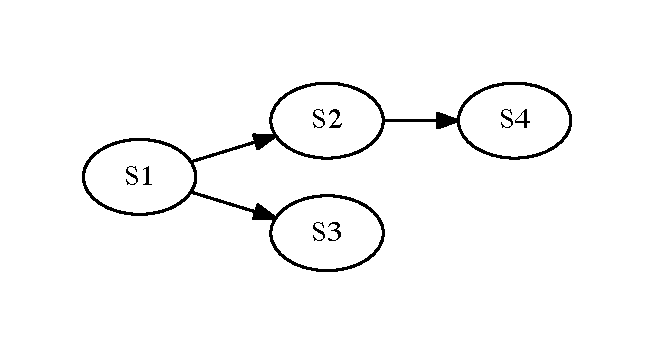
\includegraphics[width=4cm]{graphs/exemple1}}
\caption{ Precedence graph between four abstract services. }
\end{figure}
\end{example}

Each abstract service may be realized with several possible concret services. When abstract service orchestration is defined, we need to choose for each abstract service an appropriate concrete service that performs the corresponding service.  in SOA architectures, workflow  describe how activities or tasks should be carried out. We denote by concrete workflow the possible  concrete services organisation in order to realize an end to end user service in a respect to a given abstract service orchestration.  In the e
\begin{figure}[htpb]
\centering \fbox{ 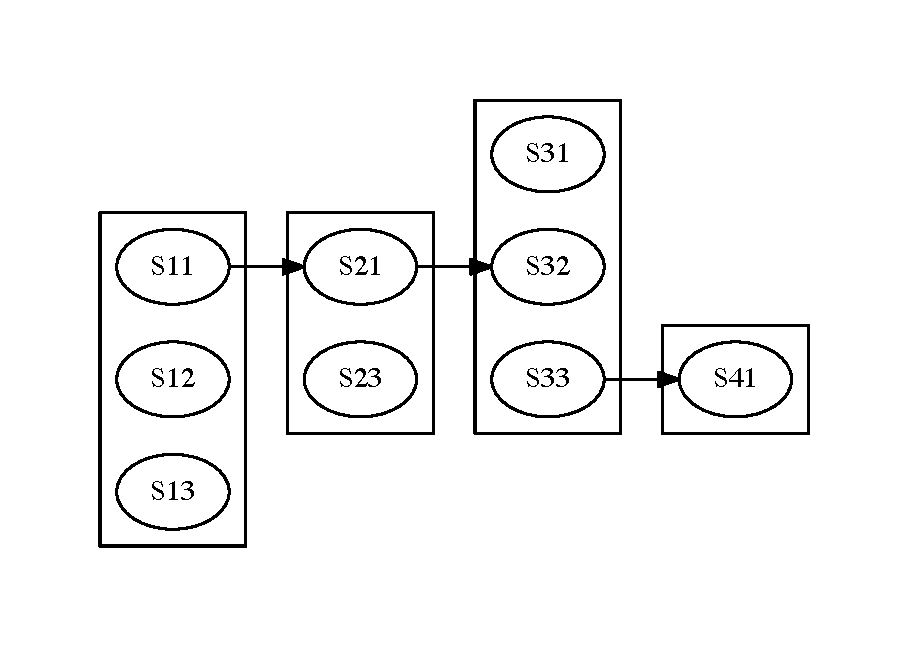
\includegraphics[width=5cm]{graphs/exemple2}}
\caption{ The concrete workflow $(S_{11},S_{21},S_{32},S_{41})$ is a possible organisation to realize the orchestration given in figure \ref{figureOrchestration}. }
\end{figure}


Let consider $f$ as a global objective function for the end-to-end service. This function optimizes $Q$ criteria list according to some fixed constraints. Let us consider $\psi(S)$ be the $M$ possible abstract service orchestrations in which we denote the $k$-th possible orchestration as $\psi_k$ (for $k\in\{1..M\})$. Thus, $F_{\psi_k}$ indicates the evaluation function of all possible concrete service concatenation of $\psi_k$.%dans le cas ou les services abstrait sont independent, le cout du critère global s'obtient par l'addition des critère de chaque service abstrait


For each $k\in\{1..M\}$,  to obtain $F_{\psi_k}$ it is necessary to select the best concrete service concatenation according to the $Q$ criteria between concrete services in the given $\psi_k$ orchestration according to predefined optimisation function $\varphi_{ki,(k \in\{1, \dots,M\}, i \in\{1,\dots,n_k\}}$ between criteria of $Q$. \\ % dans le cas ou la concatenation des services abstrait n'a pas d'impact sur les critères des services concrets l'évaluation de chaque service abstrait ne dépend pas de l'orchestration donc cette étape est inutile 
Without loss of generality, %if we consider that the optimale evaluation function between two concatenated abstract services is defined as a sum between the optimal evaluation function of concrete service of each one, then 
the service selection problem can be defined as follow: $$ Find ~the ~evaluation~ function~ f~ as~ the~ best ~value ~of ~ F_{\psi_k} $$


\begin{example} Let us consider a problem with three abstract services $\{S_1,S_2,S_3\}$ with a single possible orchestration $\psi(S_i)_{I\in\{1..3\}}=\psi_1$, such that $\psi_1$ represents a serial $(S_1,S_2,S_3)$ orchestration (we execute first concrete services of $S_1$, then $S_2$ ones and finish with $S_3$ concretes services). Let us consider a problem with two evaluation criteria $Q=\{q_1,q_2\}$ (for instance, throughput and service time response) such that the concrete services evaluation function to be optimized is defined as linear combination between these criteria: $\varphi(q_1,q_2)= w_{i1}.q_1+w_{i2}.q_2$ for each abstract service $S_i$. \\
In this case, the problem can be summarized as finding an appropriate weighted parameters $w_{ij}$ by solving the following maximization problem:
$$ max(\sum_{i=1}^{i=3} w_{i1}.q_1+w_{i2}.q_2)$$
\end{example}
However, from operational point of view, the evaluation of the quality of concrete services is estimated over concrete service executions (instances) over the time. Additional sub-problems must be solved before optimizing the previous problem among which: how to solve the service composition problem without any knowledge about user preferences criteria. 
%{\it Find the optimal concrete service permutation according to a given evaluation function on temporal concrete services instances.} \\
%This problem requires the resolution of a set of sub-problems among which:
%\begin{itemize}
%\item 
%\item
%\item
%\end{itemize}
As is shown in related work section, several works are done using various approaches. However some additional constraints make this problem more difficult. The main constraint concerns the fact that no preferences are given on the components of the evaluation function. We propose in our work to learn this preferences from data by using an original approach based on discrete time vector valued MDP especially to estimate quality of service criteria weights for any abstract service orchestration without using user quality of service preferences.\\
 In section \ref{dataset} we present a dataset used for our experiments and our considered assumptions. Section \ref{MDP} summarizes Vector-valueted decision process (VMDP) needs for our work and gives the VMDP service selection formulation according to the context presented in section \ref{dataset}.  Section \ref{MDP-algo} presented used algorithms to solve the problem and gives some complexity issues. Obtained results are given in section \ref{results}. 
 
\subsection{On the global problem complexity}
Without loss of generality, let us consider the problem with $n$ abstract services $S_1,\dots, S_n$, such that each abstract service $S_i$ can be concretized by exactly $m$ possible concrete services and there is no explicit constraint between concrete services. We assume also than each end-to-endThe purpose of this section is to enumerate the number of end-to-end concrete service combination in order to evaluate the quality of service of each combination and then select the best one according to given user or computed preferences.

As far as we know, there is no existing work dealing with this enumeration problem. The main idea of this enumeration is first to evaluate the worst complexity case and then to find a best way to reduce the quality of service evaluation time cost by performing evaluations by equivalence groups for example.  We will present some typical  cases for which we have an exact enumeration and we will give a lower bound for the general case.

\subsubsection{Complexity when there exist a total order between abstract services}
Let us consider $S_1,\dots, S_n$ this order.  Since that each $S_i$ can be realized by $m$ possible concrete services, the possible number of realizations for each order is $n^m$. If there is no additional constraint between abstract services, the number of abstract services permutations will be $n!$. Therefor the  number of  concrete services realizations will be $n!*n^m$.

\subsubsection{Complexity when all abstract services are realized in parallel}
In this case there exists only one possible combination between abstract services. For this alone combination, there exists  $n^m$ possibles realizations. 

\subsubsection{Only two abstract services are realized in parallel}
Let us consider $i$ the number of abstract services realized in parallel and $St(n,i)%=\frac{1}{i!}\sum_{j=0}^{j=i}(-1)^j \binom i j (i-j)^n 
$ the Stirling number of the second kind\footnote{$St(n,i)$ count the number of ways to partition an n-element set into i equivalence classes. It satisfy the recursion formula: $S(n,i)= S(n-1,i-1)+i*S(n-1,i)$.}. \\
If we consider the case where there is two and only two abstract services realized in parallel for a given one total order configuration of abstract services, the number of equivalent classes of length $(n-1)$ is given by $S(n,2)=2^{n-1}-1$. %\frac{1}{2!}\sum_{j=0}^{j=2}(-1)^j \binom 2 j (2-j)^n
 Therefor the number of abstract service configurations will be $(2^{n-1}-1)*(n-1)!$. In this particular case, for each abstract service configuration there is at most $2*(n-1)^m$ possible realizations. We conclude that the possible number of configurations is $2*(n-1)^m*(2^{n-1}-1)*(n-1)!$.
\subsubsection{The complexity in the case of $k$ equivalent classes}
The number of abstract services equivalent classes if given by $S(n,k)$. The number of abstract service configurations will be $S(n,k)*k!$. \\
Let us denote by $CSC$, the number of concrete services configurations and $CSC_k$ the number of concrete service configuration with $k$ equivalent classes.  In this case it is possible to compute upper and lower bound of possible configurations as follow: In all cases, the cardinal of all set of equivalent classes of abstract services is greater or egaI to $m$ and for the case of $k$ equivalent classes the set greatest cardinal is $(n-k+1)$. Thereby, it's possible to give the follow bounded result: $m^k*S(n,k)*k! \leq CSC_k \leq ((n-k+1)*m)^k*S(n,k)*k! $

From all that, it is possible to bound the realization number in general case as follow:
$  \sum_{i=1}^{i=n}  (m^i*S(n,i) *i! ) \leq CSC \leq  \sum_{i=1}^{i=n}  (((n-i+1)*m)^i*S(n,i)*i!)$.

$$\ CSC \geq \sum_{i=1}^{i=n}  (m^i*\sum_{j=0}^{j=i}(-1)^j \binom i j (i-j)^n)$$
$$CSC \leq  \sum_{i=1}^{i=n}  (((n-i+1)*m)^i*\sum_{j=0}^{j=i}(-1)^j \binom i j (i-j)^n) $$
% les bornes sont larges, elles peuvent être améliorer. pour une classe d'équivalence l'ordre de grandeur du débordement de la borne par rapport à la valeur exact est  de l'ordre de (n-k-1)^k 

%permutation complete avec égalité : un seul groupe, tous les groupes possibles.
% add some complexity results : maybe use Stirling number of the second kind
% le nombre d'orchestrations serait de n! Si pas de superposition d'états. Ici rechercher la complexité dans le cas ou les états peuvent se superposer. 



\section{MDP Problem Formulation}
 Markov Decision Processes (MDPs) are the suitable models for sequential decision problems such as QoS decomposition problems. In this section, we demonstrate how to use the MDP model to model and solve the service composition problem. We are looking for an optimal  QoS-selection corresponding the user's preferences on qualities of services. Since the user's preferences among service qualities are unknown, we consider the problem as a multi-objective service composition under uncertainties. For this reason, we utilize a partially known MDP model and more particularly a Vector-valued MDP (VMDP) model.  Before getting into details, it is required to describe some preliminary properties and definitions as follows. 

\begin{property}
A \textbf{Concrete Service} $S_{ij}$, or a concrete service executed by an actor with or without time reference properties can be summarized on two parts: functional properties and non-functional ones.

\begin{itemize}
\item Functional : $S_{ij}$ is under the form of transaction function Action$(S_{ij})$ that takes an input data vector InputData$(S_{ij})$ to produce an output data vector OutputData$(S_{ij})$ 
\item Non-functional : is defined by a QoS attributes vector QoS$(S_{ij})$, the energy profile EProf$(S_{ij})$, etc.  
\end{itemize}

\end{property}

\begin{property}
An \textbf{Abstract Service} $S_i = \{ S_{i1}, \cdots, S_{in_i} \}$ is a class of $n_i$ concrete services with similar functional properties. That means they have the same input data vector and output data vector, but their nonfunctional properties are different. 
\end{property}
In the rest of this section, we will explain how various classes of abstract services, each one including many concrete services can be modeled as a Vector-valued MDP. For the sake of simplicity, we will demonstrate the modeling process step by step. 

\subsection{Vector-valued Markov Decision Process}
Referring to Section~\ref{section:problem-formulation} invoking each concert service in a time step $t$ produces different quality of services. Reminding Example~\ref{example:DB}, invoking concrete service $3104$ for abstract service $19994$ at time $5$ gives two different values for the response time and throughput: $Q(s_{ij}) = (\text{rt}(S_{ij}), \text{tp}(S_{ij}))$. 

\begin{definition}
Formally, a \emph{Discrete-time Markov Decision Process (Discrete-time MDP)} \cite{timeMDP} is defined by a tuple $(T, S, A, P_t(.|s,a), r_t)$ where:

\begin{itemize}
\item[-] $T=0,\cdots, N$ are the decision time steps at which the decisions are made\footnote{time steps can be days, hours, minutes or any time interval}. 
\item[-]States: $S$ is a finite set of States
\item[-] Actions: $A(s)$ is a finite set of actions that agent can select to interact with the environment.
\item[-] State Transition Probability Distribution: $P_t(s'| s,a)$ encodes the probability of going to state $s'$ when the agent is in state $s$ and chooses action $a$.
\item[-] Reward Function: $r_t : S \times A \longrightarrow \mathbb{R}$. $r_t(s,a)$ quantifies the utility of performing action $a$ in state $s$ at the $t$ time step.
%\item[-] Discount Factor: $\gamma \in [0,1)$ indicates how less important are future rewards in compared to the immediate ones. 
%\item[-] Initial State Distribution: $\beta : S \longrightarrow [0, 1]$ indicates that the probability that the agent starts her interactions with the environment in state $s$ is $\beta(s)$.
\end{itemize}

\end{definition}

A \emph{Decision rule} $d_t$ is a function depends on time $t$ that defines what action $d_t(s) \in A(s)$ at time $t$ the agent should select. By assuming $N$ number of time steps, we define \emph{policy} $\pi = (d_1, \cdots, d_{N-1})$ as a sequence of $N-1$  decision rules. The policy is stationary if: $\forall \; t \in \{1, \cdots, T \} \; d_t = d$. 

A solution for MDP is a policy $\pi: S \longrightarrow A$ that associates an action to each state. Normally, policies are evaluated by a value function $v^{\pi} : S \longrightarrow \mathbb{R}$. The value function is computed recursively using several recursive functions: %namely \emph{Bellman equations}:
\begin{equation}
v^{\pi}_N(s) = r_N(s, \pi(s)) \;\; \forall s\in S_T
\end{equation}

where $S_T$ is the set of terminal states as a subset of all states $S$: $S_T \subset S$. Remind that there is no action decision in  $S_T$ as the set of terminal states. For the rest of time steps $t<T$, the value function is defined as:

\begin{equation}\label{eq:value-func}
v^{\pi}_t(s) =  r_t(s,\pi(s)) + \gamma \sum_{s' \in S} P_t(s'|s,\pi(s)) v^{\pi}(s')
\end{equation}

where $\gamma$ is a discount factor and we have $ 0 < \gamma \leq 1$. Therefore, the preference relation among policies is defined as below:

\begin{equation}
\pi \succeq \pi' \Leftrightarrow \forall s \in S \; v_0^{\pi}(s) \geq v_0^{\pi'}(s)
\end{equation}

An MDP solution is an \emph{optimal policy}, that is the highest policy with respect to the other policies and the preference relation $\succeq$, i.e. $\pi *$ is an optimal policy if: 

\begin{equation}
\pi^* \text{s.t.} \; \forall \; \pi, \; \pi^* \succeq \pi
\end{equation}

To find such a policy/workflow, we can use a dynamic programming, namely \emph{Bellman Equation}. 
\begin{equation}
v_N^* = r_N(s) \; \forall s\in S_T
\end{equation}
%
and for all $t= 1, \cdots, N-1$ and $s \in S$, the value of the optimal policy is computed as:
\begin{equation}\label{eq:bellman}
v_t^*(s) =\text{max}_{a \in A(s)} \left \{ r_t(s,a) + \gamma \sum_{s' \in S} P(s'|s,a) v_{t+1}^*(s') \right \} 
\end{equation}

For the sake of simplicity, we define Q-value function on state $s$ and action $a$ at time step $t$ as:

\begin{equation}
Q_t(s,a) = r_t(s,a) + \gamma \sum_{s' \in S} P(s'|s,a) v_{t+1}^*(s')
\end{equation}
In the other hand, the optimal policy is the policy that selects action $a^*$ at stage $t$ from the following:
\begin{equation}\label{eq:opt-action}
a^*_t \in \text{argmax}_{a \in A(s)} \left \{ Q_t(s,a) \right \} \; \text{ for } t=1 \cdots N-1
\end{equation}

Sometimes, selecting an action in a given state may have several effects instead of only one value. It means, by extending the discrete-time MDP to a discrete-time vector-valued MDP ( discrete-time VMDP), we have: 

\begin{definition} \cite{alizadeh:hal-01358345}
A \textbf{discrete-time Vector-valued MDP (discrete-time VMDP)} is defined by a tuple $ (T, S, A, P_t(.|s,a), \bar{r}_t)$ where the vector-valued reward function $\bar{r}$ is defined on $S \times A$ and $\bar{r}(s, a) = ({r_1}_t(s,a), \cdots, {r_d}_t(s,a)) \in \mathbb{R}^d$ is the vector valued reward defined by $\bar{r}$ in state $s$ and action $a$. 
\end{definition}

Notice that the VMDP is another form of Multi objective MDP. That means, $d$ is the number of objectives in the environment while each element $i$ in reward vector $\bar{r}(s, a)$ indicates cost of the $i$-th objective in the model by selecting action $a$ in state $s$. 

\subsection{MDP for Service Compositions}

By modeling the service composition as a discrete-time VMDP, we can 
compute the best selected work-flow respecting user preferences on quality of services attributes. Note that we are allowed to communicate with users in order to get information about their priorities and preferences. 

We use discrete-time VMDP modeling to select the optimal concrete service in each abstract service w.r.t time stage $t$. For the sake of simplicity, this model is noted as discrete-time VMDP-Service Composition (discrete-time VMDP-SC) which is introduced in the rest of this section (see \cite{Wang2010,Mostafa2015}). 

\begin{definition}
A \textbf{VMDP-Service Composition (VMDP-SC} is a tuple $(T, AS, CS, P_t(.|as,cs), \bar{r}_t, AS_T)$, where  

\begin{itemize}
\item[ -] $T= 1, \cdots N$ is a total number of time stages. 
\item[-] $AS$ is a finite set of abstract services.
\item[-] $\{S_{ij}\}_j$ is the set of available concrete services for the abstract service $S_i \in AS$.
\item[-] $P_t(S_j | S_i, S_{ik} )$ is the probability of invoking the concrete service $S_{ik}$ for abstract activity $S_i$ and resulting in the abstract activity $S_j$.
\item[-] $ \overline{Q}_t: AS \times CS \longrightarrow \mathbb{R}^d$ is a reward function. The $\overline{Q}(S_i, S_{ik})$ reward is the generated Q vector value after invoking $S_{ik}$ in $S_i$ at time step $t$. ( Notice that $d$ is the number of quality of service attributes and we have $\overline{Q}_t(S_i, S_{ik}) = ({q_1}_t(S_i, S_{ik}), \cdots, {q_d}_t(S_i, S_{ik}))$ ). 
\item[-] $AS_T$ is the set of terminal services. It means the execution of the service composition terminates by ending in one of these states.
%\item[-] $\beta(sa)$ represents the probability of starting abstract activity in abstract service $sa$. Remind that $\sum_{sa \in SA} \beta(sa) = 1 $. ({\color{red} if I remove $\beta$, I will use the MDP model with start abstract services such as \cite{DBLP:journals/tase/KhanoucheACKY16}. })
\end{itemize}
\label{def:vmdp-sc}
\end{definition}

The solution for QoS-aware service selection is defined as a policy in VMDP-SC model.

\begin{definition}
A \textbf{policy service composition} $\pi: AS \longrightarrow SC$ is a function that defines which concrete service should be invoked for each abstract service in order to give the best trade-offs among multiple QoS attributes. 
\end{definition}

This policy is known as a workflow or plan in the IOT literature. Since reward values in MDP-SC are the $Q$ vectors for each concrete services, each policy should be evaluated with a vector function (see Equation~\ref{eq:value-func}):
\begin{equation}
\bar{v}_t^{\pi}(S_i) = \overline{Q}_t(S_i, \pi(S_i)) + \gamma \sum_{S_j \in S} P(S_j | \pi(S_i), S_i) \bar{v}_{t+1}^{\pi}(S_j)
\end{equation}

By assumption, this function is called \emph{Q vector valued function}. Now, comparing two workflows/policies boils down to comparing two vectors. The optimal workflows satisfying various users with different preferences among the QoS attributes are not the same. 

\begin{example}
Give an example from the data base to explain the reason of last written phrase.
\end{example}

Thus, we need a model that presents the user preferences over quality of services attributes. 
\begin{example}
Another examples that shows the relation between user preferences on the qos attributes.
\end{example}

For this reason, we define user preferences over the QoS attributes as a linear combination of the quality of service attributes. In fact, if any user gives a  weight to each attribute, the dependency between the users' weights and quality of service attributes is defined as below:

\begin{multline}
Q_t(S_i, S_{ij}) = \sum_{k=1}^d \bar{w}_k {q_k}_t = \bar{w} \cdot \overline{Q}(S_i, S_{ij}) \\
\forall t = 1, \cdots, N
\end{multline}

where $\bar{w} = (w_0, \cdots, w_d) $ is a weight vector, indicating the user preferences on the QoS attributes such that 
\begin{equation*}
\sum_{i=1}^d w_i = 1
\end{equation*}

If the user preferences on the QoS attributes is given, the optimal workflow can be computed easily. Since defining a weight to each QoS attribute is not obvious by users ({\color{red} we need stronger motivation related to IOT}), we assume that $\bar{w}$ is unknown and try to find the best workflow/policy/plan by querying users when it is necessary. ({\color{red} this phrase should be rephrased and very strong motivation should be added to this part.}). 

To compare workflow vector values with each other, we consider first, the unknown weight vectors are confined in a $d-1$ dimensional polytope $W$ such that:
\begin{equation}
W = \{ (w_1, w_2, \cdots, w_d) \; | \; \sum_{i=2}^d w_i \leq 1 \; \text{and} \; w_1 = 1-\sum_{i=2}^d w_i \}
\end{equation}

To compare Q vector values with each other, we can use three different comparison methods.

Assume $\bar{v}^a = (a_1, \cdots, a_d)$  and $\bar{v}^b = (b_1, \cdots, b_d)$ are two $d$-dimensional vectors representing expectation of sum of QoS values for two workflows $a$ and $b$. 

\begin{itemize}
\item[-] the most natural comparison method is \emph{pareto comparison} that defines:
\begin{equation} \label{eq:pareto}
\bar{v}^a \succeq_P \bar{v}^b \Leftrightarrow \forall \; i \; a_i \geq b_i
\end{equation}\label{eq:kdom}
\item[-] \emph{Kdominance comparison} defines $\bar{v}^a$ is more preferred than $\bar{v}^b$ if, it is better for any $\bar{w}$ in polytope $W$:
\begin{equation}
\bar{v}^a \succeq_K \bar{v}^b \Leftrightarrow \forall \; \bar{w} \in W \; \bar{w} \cdot \bar{v}^a \geq \bar{w} \cdot \bar{v}^b
\end{equation}\label{eq:queryuser}
\item[-] query this comparison to the user, i.e. $\bar{v}^a  \succeq_q \bar{v}^b$. 
\end{itemize} 

Remind that, the Kdominance comparison is a linear programming problem. it means, $\bar{v}^a  \succeq_K \bar{v}^b$ satisfies, if there is a non-negative solution for the following LP:
\begin{equation}
\left\{
\begin{array}{ll}
\text{min} \; \bar{w} \cdot (\bar{v}^a - \bar{v}^b) \\
\text{subject to } \; \bar{w} \in W
\end{array}
\right.
\end{equation}
If there is no non-negative solution for two comparisons $\bar{v}^a  \succeq_K \bar{v}^b$ and $\bar{v}^b  \succeq_K \bar{v}^a$, these two vectors are not comparable using the Kdominance. 

In the rest of this paper, we will explain how to find the optimal policy/workflow that gives the best trade-off among multiple QoS criteria, satisfying the user preferences on QoS attributes by querying users very few times. % Since we are interested in computing the best match for each agent regarding her preferences, our algorithms queries the agent when it is required. %Therefore, the proposed queries to the agent get the partial information on their preferences on the QoS attributes.  

In this section, we propose an Algorithm namely \emph{Interactive Value Iteration for Service Composition (IVI-SC)}. Previously, we explained how model web services as a discrete-time MDP in order to solve the service composition problem. In this section, we demonstrate, how to find the solution using the existed solutions for MDPs. Some researchers use interactive value iteration methods to find the optimal service composition respecting the user of system preferences \cite{weng:hal-00942290,alizadeh:hal-01358345}. In this paper, we modified the interactive value iteration on a finite-horizontal MDP to find the best service composition satisfying users' priorities on quality of services. 

\section{Interactive Reinforcement Learning Algorithms for the Service Compositions}

In this section we assume that an MDP model of services (VMDP-SC) with finite discrete-time is given. The services can be invoked in $T+1$ number of discrete time steps: $\{0, \cdots,T-1 \} \cup \{T\}$ where $T$ is a final empty time stage. %That means, the quality of all the invoked concrete services in time step $T$ are zero.
Since the MDP-SC objective is to find the policy that maximizes a measure of long-run expected Q vectors, we propose a backward induction method to solve the Bellman equation given in equation~\ref{eq:bellman} and finds the optimal actions given in equation~\ref{eq:opt-action} to obtain the optimal policy/work-flow. Our solution is introduced in Algorithm~\ref{algo:ivi}.

\begin{algorithm}[]
 \KwData{VMDP-SC$(T, AS, CS(), P_t, \bar{r}_t)$, a $W$ polytope of user weights on objectives, precision $\epsilon$}
 \KwResult{The optimal service selection policy for the given user. }
 $t \longleftarrow T$ \\
 $\pi_{\text{best}} \longleftarrow $ choose random policy \\
$\bar{v}_{T}(s_T) \longleftarrow (0, \cdots,0)$\footnote{zero vector of dimension $d$ where $d$ is the number of quality attributes for QoS}  $\forall s_T$ at time $T$  \\
 $\mathcal{K} \longleftarrow $ set of constraints on $W$ \\
 \While{$t \geq 0$}{
 	$t \longleftarrow t-1$ \\
	%\For{\textbf{each} $as \in AS$}{
	\For{\textbf{each} $h_t = (h_{t-1}, cs_{t-1}, as_t) \in H_t$}{
		best $\longleftarrow (0, \cdots, 0)$ \\
		%\For{\textbf{each} $cs_{t-1} \in A(as)$}
		\For{\textbf{ each } $cs \in CS(as_t)$}{
			$\bar{v}_t(as_t) \longleftarrow \overline{QoS}_t(as_t, cs) + \sum_{as'} P_t(as' | as_t, cs) \bar{v}_{t+1}(as')$\\
			$($ best $, \mathcal{K} ) \longleftarrow $ getBest(best, $\bar{v}_t, \mathcal{K}$) \\
		   	$\bar{v}_t(as_t) \longleftarrow $ best \\
		   	\If{best = $\bar{v}_t(as_t)$}{
				$\pi_{\text{best}(as_t) \longleftarrow cs}$
			}
	 }
	}
 } 
 \textbf{return} $\pi_{\text{best}}$ \\
 \vspace{0.3cm}
 \caption{How to select the best composite for each abstract service respecting user preferences on QoS attributes}
\end{algorithm}\label{algo:ivi}
%%%%%%%%%%%%%%%%%

%%%%%%%%%%%%%%%%%%%%

\begin{algorithm}[]

\KwData{finds the more preferred vector between two vectors $\bar{v}$ and $\bar{v}'$ w.r.t $ \mathcal{K}$}
\KwResult{}

\If{paretodominates($\bar{v}, \bar{v}'$)}{
	\textbf{return} $(\bar{v}, \mathcal{K})$
}
\If{paretodominates($\bar{v}', \bar{v}$)}{
	\textbf{return} $(\bar{v}', \mathcal{K})$
}
\If{Kdominates($\bar{v}, \bar{v}',  \mathcal{K}$)}{
	\textbf{return} $(\bar{v}, \mathcal{K})$
}
\If{Kdominates($\bar{v}', \bar{v},  \mathcal{K}$)}{
	\textbf{return} $(\bar{v}', \mathcal{K})$
}
$(\bar{v}_{\text{best}}, \mathcal{K}) \longleftarrow $ query$(\bar{v}, \bar{v}',  \mathcal{K})$ \\
\textbf{return} $(\bar{v}_{\text{best}}, \mathcal{K})$
\caption{\textbf{Best}: this algorithm finds the most preferred vector between two given vectors.}
\end{algorithm}\label{algo:getBest}
%%%%%%%%%%%%%%%%%%%%

In  iterative algorithm~\ref{algo:ivi}, first we assign a zero vector to the set of states (abstract services) at time step $T$. At each iteration on the abstract services, the algorithm should solve equation~\ref{eq:bellman}, using the value from the previous iteration. Notice that $h_t = (h_{t-1}, cs_{t-1}, as_t)$ indicates that by invoking a concrete service $as_{t-1}$ at time $t-1$, the system will be at concrete service $as_t$. %In the infinite horizon time, the iteration continues until the difference between successive values becomes extremely small. 
In the finite horizon time (our case), the iteration continues until either this difference becomes small enough or the horizon time steps finish. 

%%%%%%%%%%%%%%%%%%%%
\begin{algorithm}[]
\KwData{$\bar{v}, \bar{v}', \mathcal{K}$}
\KwResult{ it queries the comparison between $\bar{v}$ and $\bar{v}',$ to the user and modifies $\mathcal{K}$ according to her response.}
Build query $q$ for the comparison between $\bar{v}$ and $\bar{v}'$ \\
\If{if the user prefers $\bar{v}$ to $\bar{v}'$}{
	\textbf{return} $(\bar{v}, \{ (\bar{v} - \bar{v}') \cdot \bar{w} \geq 0 \})$
}
\Else{
	\textbf{return} $(\bar{v}', \{ (\bar{v}' - \bar{v}) \cdot \bar{w} \geq 0 \})$
}
\caption{\textbf{query}: queries the user about her preferences on existed quality of services.}
\end{algorithm}\label{algo:query}

Since the quality of services are the $d$ dimensional vectors, solving equation~\ref{eq:bellman} and finding the maximum among the vectors is not obvious. For this reason, we remind three comparison methods (presented in equations~\ref{eq:pareto}, $13$ and $14$ %~\ref{eq:kdom} and~\ref{eq:queryuser}
) and utilize function \textbf{Best} (Algorithm~\ref{algo:getBest}). This function receives two $d$ dimensional vectors with the $W$ polytope confining the user weight preferences on the quality of services. If pareto comparison does not have a solution, the Kdominance comparison method will try this comparison out. Otherwise the query function should be called (given in Algorithm~\ref{algo:query}) where the user response to the comparison between the two given vectors, adds a new constraint to the $W$. 

Algorithm~\ref{algo:ivi} finally finds the optimal policy/work-flow or service composition for the given system MDP-SC and returns back the optimal policy $\pi_{\text{best}}$. Notice that the condition $best = \bar{v}_t(as_t)$ checks if the best selected concrete service for $as_t$ has been changed regarding the previous iteration. If it was the case, the optimal concrete service should be replaced by the concrete service $cs$ which generates a better vector value for $as_t$. 
 
{ \color{red}add a part on complexity of algorithms and so on.}

\section{Performance Evaluation}

We evaluate our methods on a public available dataset containing two parameters for quality of services: response time and throughput. These are the records between $339$ users and $5825$ web services distributed worldwide \cite{Zheng2014,Zheng2015}. The dataset also includes some information about user features, service features such as countries, autonomous systems, IP dresses, latitude and longitude. In the studied data base, users execute various web services in different time slices. Practically, the information are given only for $64$ time steps. 

In this section, we explain first how to model the studied dataset as a VMDP-SC and then we will examine our algorithm on the dataset in two different approaches including the divided dataset based on the users' existed information and  a filtered version of database. 

\subsection{Model DataSet as a VMDP}
The main issue in implementing Algorithm~\ref{algo:ivi} on any database is that how to model the given set as a vector-valued MDP. In the supported dataset \cite{Zheng2014,Zheng2015}, there are several text files including wslist.txt, userlist.txt, rtdata.txt and tpdata.txt. Using the wslist.txt, we extract a list of web services and their related abstract services, if a related abstract service exist for the selected web service. In total, there are $5825$ web services and $137$ abstract services. The userlist.txt includes the information about $338$ users of different web services. The two other files rt.txt and tp.txt are consist of the data about user execution of web services in $64$ different time steps on response time and throughput respectively. The point is that, they present the related results of $142$ system users. Each invoked web service by a special user has two parameters for measuring the service quality: response time and throughout. 

\begin{figure}[t]
\label{fig:seq-mdp}
\centering
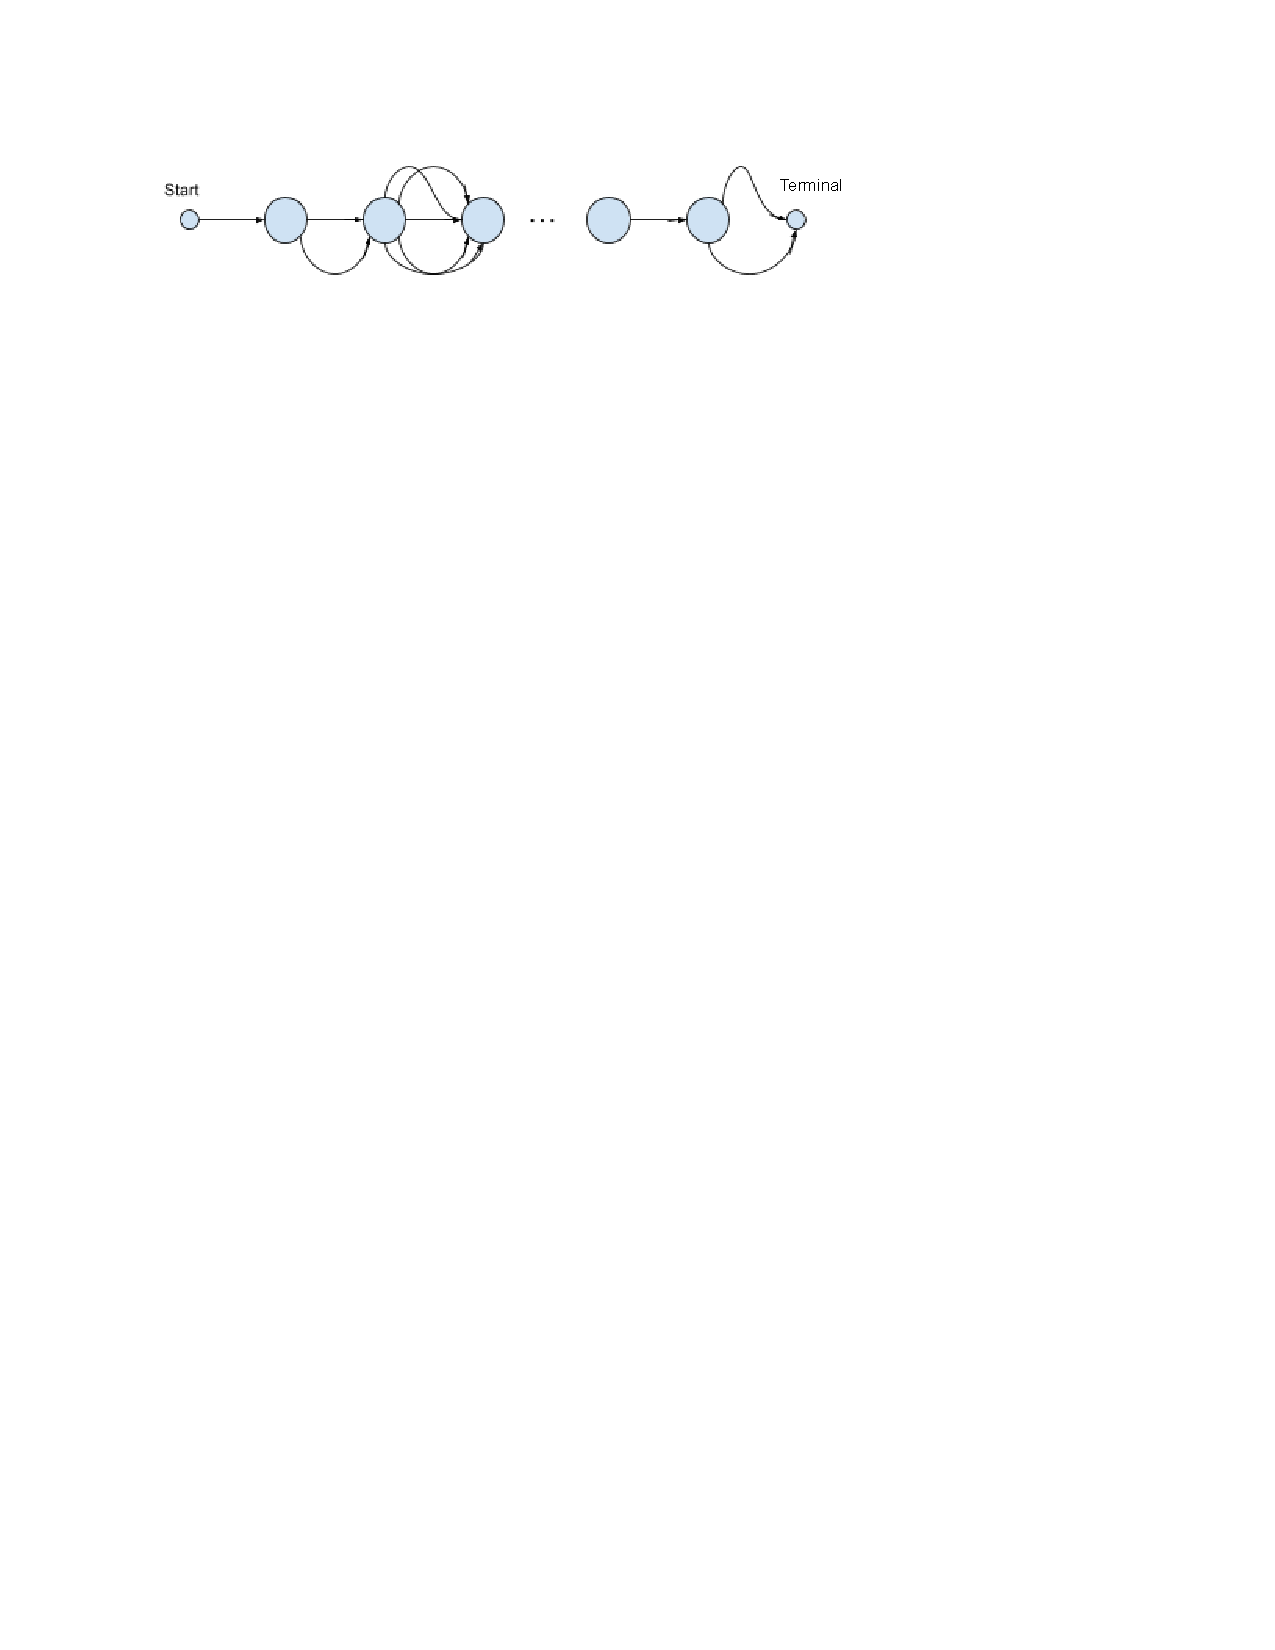
\includegraphics[width=10cm]{graphs/seq-mdp}
\caption{A sequential form of abstract service connection}
\end{figure}

\begin{figure}[t]
\label{fig:par-mdp}
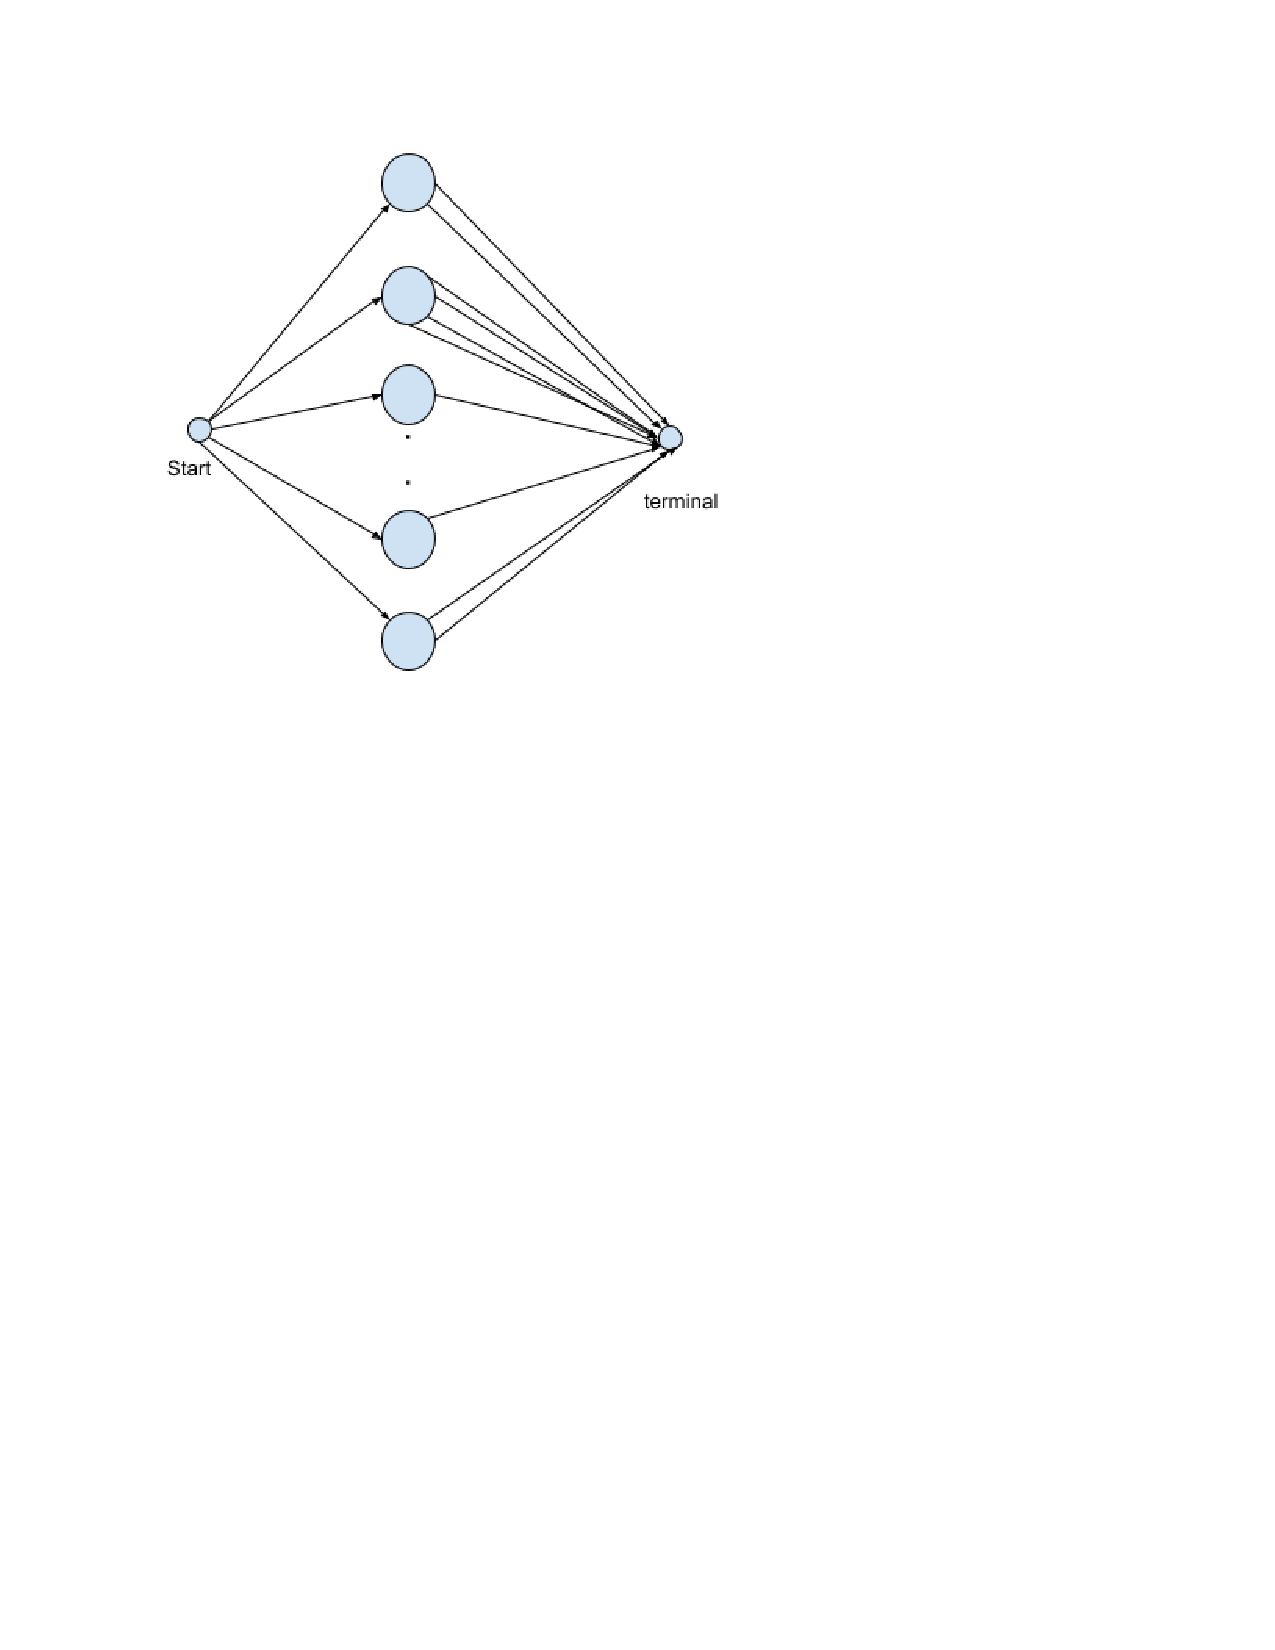
\includegraphics[width=8cm]{graphs/par-mdp}
\caption{A parallel form of abstract service connection}
\centering
\end{figure}

According to the extracted information from the database and VMDP-SC definition (see~\ref{def:vmdp-sc}) we have:
\begin{itemize}
\item[-] number of episodes:  $N=64$
\item[-] $137$ number of abstract services 
\item[-] $5825$ number of concrete services (in our case web services)
\item[-]  The transition function and terminal states depends on the proposed model or relation among the abstract services. 
\begin{itemize}

\item[1] For the sequential model (see Fig~\ref{fig:seq-mdp}) the start sate is an empty state and connected to the first selected abstract service in the model. While the terminal state is an empty state to indicate the MDP is a finite horizon one. The transition probability $P_t(S_j | S_i, S_{ik})$ is $1$, if web service $S_{ik}$ is invocable for abstract service $S_{i}$(according to our database) and abstract service $S_j$ is the next demanded service in our selected sequential MDP model for all time steps $t=0 \cdots 63$. 

\item[2] For the parallel model (see Fig~\ref{fig:par-mdp}), the start and terminal states are the empty sates such that the start state has access to all abstract services and the abstract services are connected to the terminal state based on the possible web services for each one. In this case, $P_t(S_j | S_i, S_{ik})$ is $1$ if $S_j$ is the terminal state, otherwise it is $0$ for all time step $t = 0, \cdots, 63$. 
\end{itemize}

\item[-] and the $\overline{Q}_t$ function is built based on the extracted data on web services and their two qualities (response time and throughout).
\end{itemize}

\subsection{Classified Dataset}

\subsection{Filtered Dataset}
\red{lambdas should be replaced by $\bar{W}$ weight vectors in the tables.}

\begin{table}
\begin{tabular}{ l | c | }
  user & weight vector \\
  \toprule
   $\bar{W}_1$ & $[0.07075913789991828, 0.9292408621000817]$ \\
   $\bar{W}_2$ & $[0.8573741847324399, 0.14262581526756013]$ \\
   $\bar{W}_3$ & $[0.1696287781131175, 0.8303712218868825]$ \\
   $\bar{W}_4$ & $[0.6451844883834318, 0.3548155116165682]$\\
   $\bar{W}_5$ & $ [0.18190820427369447, 0.8180917957263055]$\\ 
 \end{tabular} 
 \caption{The weight vectors for $5$ random system users.} 
 \label{table:weights}
\end{table}

Our dataset is a real database generated by observing various users using enormous number of web services. We notice that all provided data inside database are not useful. After extracting all web services and their related abstract services from wslist.tx file, and getting the quality of web services of two files tp.txt and rt.txt, we recognize that there is no information on some web services related to some abstract services. For this reason, we remove the abstract services without any information on their related web services. 

\begin{figure}[t]
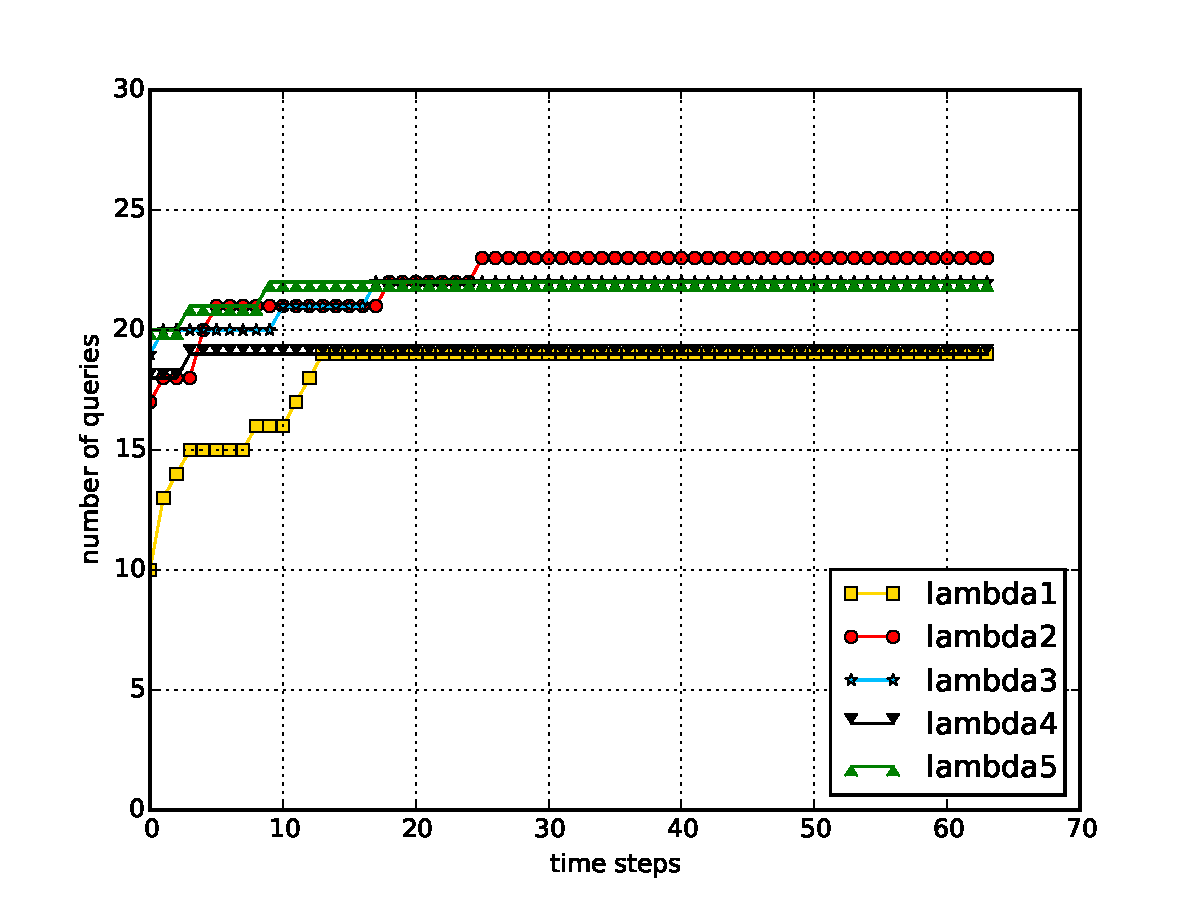
\includegraphics[width=8cm]{graphs/query-complete}
\caption{This figure shows the number of queries proposed to the user during each time step. The weight preferences are based on table~\ref{table:weights}.}
\centering
\label{fig:queries-vs-timestep}
\end{figure}


In order to evaluate our algorithms performance, we have observed the results for 5 different system users with various preferences on service qualities: response time and throughput. The user weights vector ($W$) on service qualities is given in table~\ref{table:weights}. Notice that the weight preferences on quality of services are unknown to our algorithms. We keep mention them here, because they are required for the rest of experiments. 

Figure~\ref{fig:queries-vs-timestep} demonstrates how we communicate with users during $64$ time steps. As it can be seen in this figure, we don't ask more than 23 queries to the users with various preferences on quality services. The number of communications with users are important because we can not interrupt users with too many questions. 

 
%%%%%%%%%
\begin{figure}[t]
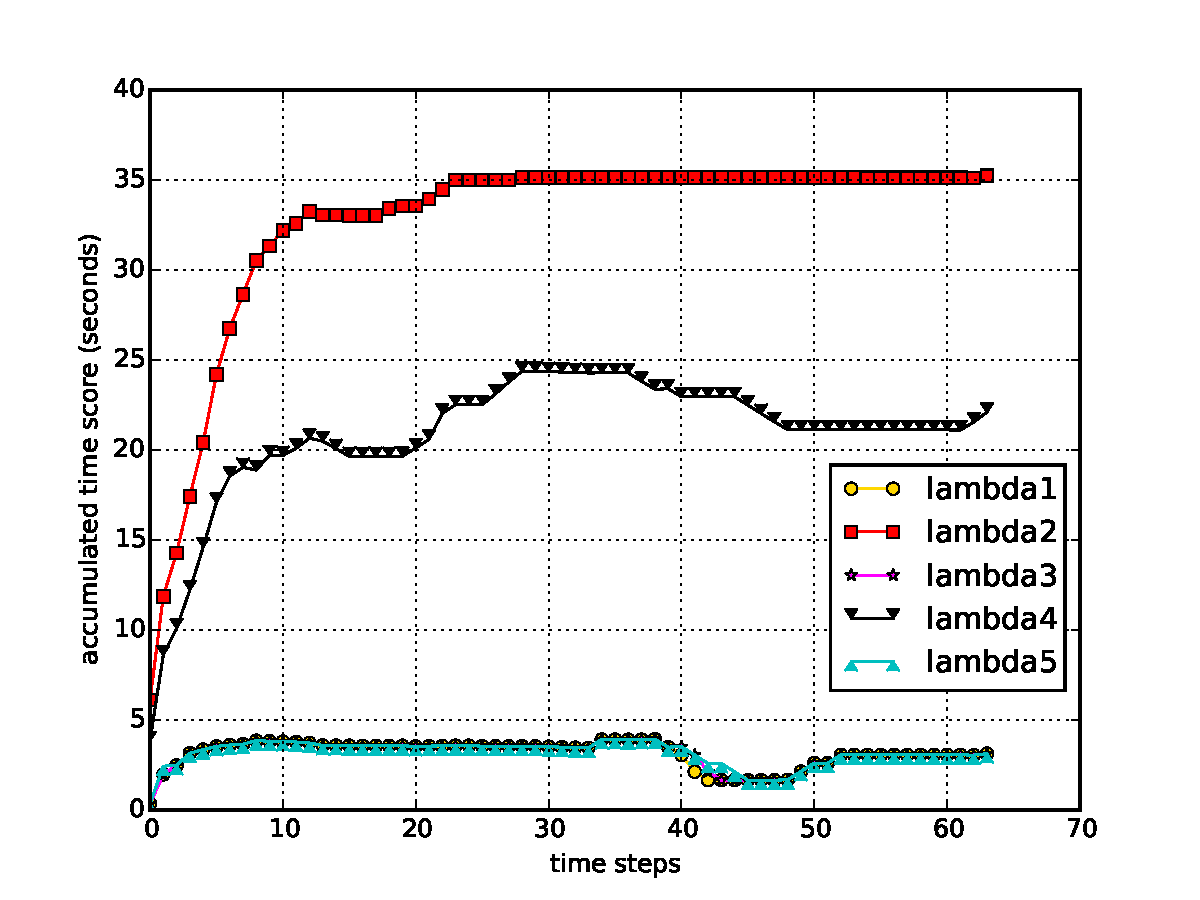
\includegraphics[width=8cm]{graphs/rt_step}
\caption{This figures demonstrates how the accumulated response time increases during each time step. The weight preferences are based on table~\ref{table:weights}.} 
\centering
\label{fig:rt-vs-timestep}
\end{figure}
%%%%%%%

\begin{figure}[t]
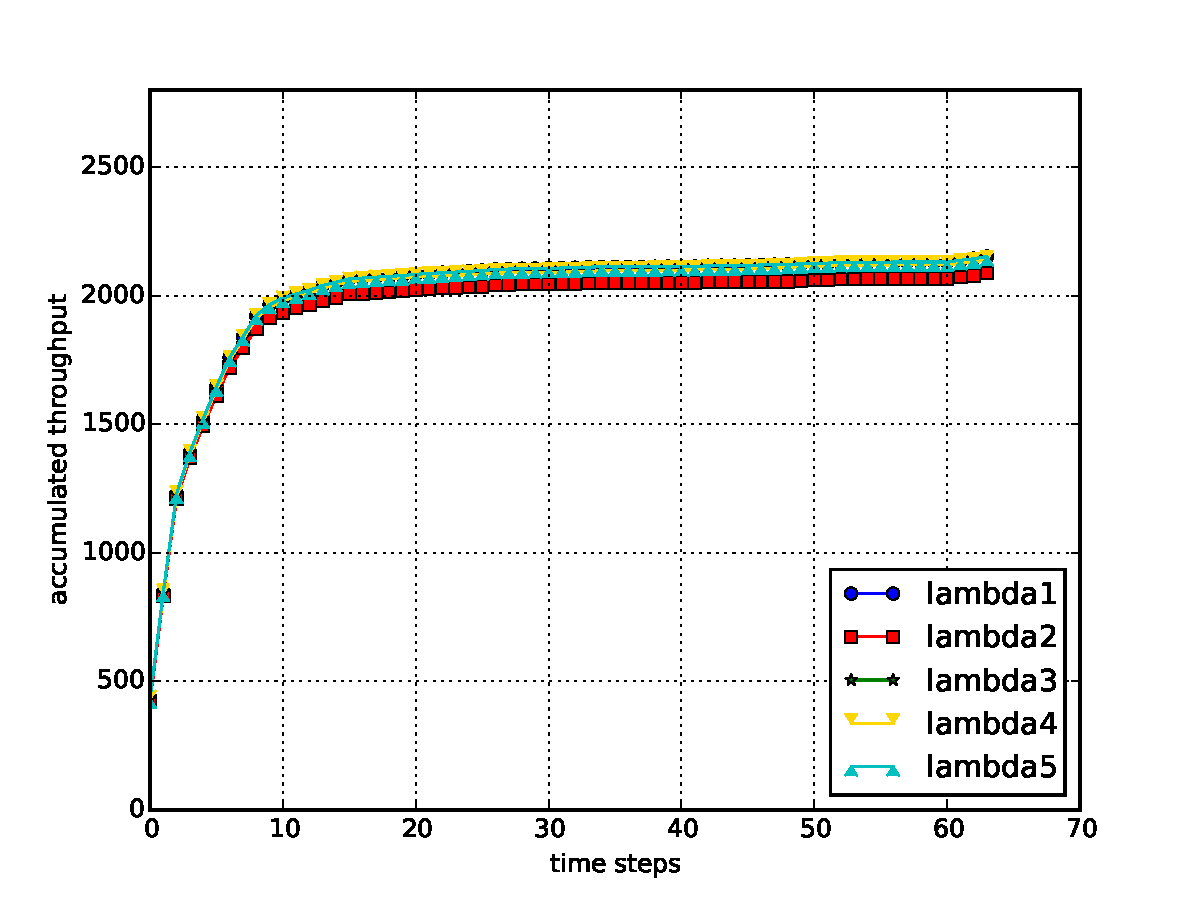
\includegraphics[width=8cm]{graphs/trough_step}
\caption{this figures demonstrates how the accumulated throughout increases during each time step. The weight preferences are based on table~\ref{table:weights}.}
\centering
\label{fig:trput-vs-timestep}
\end{figure} 

On the other hand two Figures~\ref{fig:rt-vs-timestep} and~\ref{fig:trput-vs-timestep} show how service qualities response time and throughput respectively change with respect to time step for the $5$ given user types. Figure~\ref{fig:rt-vs-timestep} indicates that three users with $\bar{W}_1$, $\bar{W}_3$ and $\bar{W}_5$ weight preferences have the similar changing in their response time evolution. While $W_2$ causes the highest computed response time. In the other hand, Figure~\ref{fig:trput-vs-timestep} shows that all tested preferred weights accumulates with almost the same steep.

We are interested in the optimal workflow i.e. which concrete services for each abstract service should be selected in order to maximize the service qualities satisfying user weight preferences. Therefore Table\ref{table:ivi-vs-axact} observes the differences between the proposed optimal workflow by algorithm \ref{algo:ivi} and an exact solution. Remind that the exact workflow is calculable by taking the weight into account and using a classical approach on MDPs such as Value iteration method~\ref{Sutton1998}.  In VMDP formulation (see \ref{def:vmdp-sc}) the reward values are vectors, but knowing the user weights $\bar{W}$, transfers the quality vectors to the qulaity values: $\bar{W} \cdot \bar{Q}$. For this reason, the value iteration is applicable on MDPs service compositions. Table\ref{table:ivi-vs-axact} compares the workflow proposed by algorithm~\ref{algo:ivi} and the exact workflow computed by value iteration method~\cite{ARASI2017}. It can be seen that the computed optimal workflow by our approach is almost the same as the exact computed workflow for the $5$ user preferences types except very few number of services. This guaranties the accuracy of our approach. 

\begin{table}[ht]
\caption{This table demonstrates how each predicted policy from algorithm \ref{algo:ivi} is close to the optimal workflow when the $\bar{\lambda}$ is known.}
\centering
\resizebox{\columnwidth}{!}{%
\begin{tabular}{lc|cc||cc||cc||cc||cc||c}
\hline
 & &  \multicolumn{2}{c||}{lambda 1} & \multicolumn{2}{c||}{lambda 2} & \multicolumn{2}{c||}{lambda 3}  & \multicolumn{2}{c||}{lambda 4} & \multicolumn{2}{c||}{lambda 5}\\
\hline
Services & \shortstack{ \tiny{number} \\ \tiny{of WS}} &IVI& Exact & IVI & Exact & IVI & Exact & IVI & Exact & IVI & Exact \\
\hline
AS5786&3 & \cellcolor{red!40} 2212 & \cellcolor{red!40} 2214  &  \cellcolor{blue!40} 2213 & \cellcolor{blue!40}2214 & \cellcolor{red!40} 2212&  \cellcolor{red!40}2214 & \cellcolor{blue!40} 2213 &  \cellcolor{blue!40}2212 & \cellcolor{green!40} 2212 & \cellcolor{green!40} 2214 \\
AS1659&1 & 2585 &2585 &2585  & 2585 & 2585 & 2585 & 2585 & 2585 & 2585 &2585 \\
AS680&44 &\cellcolor{red!40} 1398&\cellcolor{red!40} 1401& \cellcolor{blue!40}1398 & \cellcolor{blue!40}1401  &  \cellcolor{red!40}1398 & \cellcolor{red!40} 1401 & \cellcolor{blue!40}1398 & \cellcolor{blue!40}1401 & \cellcolor{green!40}1398 &\cellcolor{green!40}1401 \\
AS73& 5 &3914&3914  & 3912 & 3912 & 3914 & 3914 & 3912 & 3912 &3914  &3914 \\
AS156&2  &4180 &4180  & 4179 & 4179 & 4180 & 4180 & 4179 & 4179 & 4180 &4180 \\
AS559&2 &None  &None &  None&None  & None & None & None & None & None &None \\
AS19262& &3900 &3900  &  3900&3900  & 3900 & 3900 & 3900 & 3900 &3900  &3900 \\
AS553&2 &1466 &1466  &  1448&1448  & 1466 & 1466 & \cellcolor{blue!40}1448 & \cellcolor{blue!40}1466 &  1466&1466 \\
AS2852&2  &920 & 920  & 920 & 920 & 920 & 920 & 920 & 920 & 920 &920 \\
AS3112& &None  & None & None & None & None & None & None & None & None &None \\
AS760&4  &91 & 91&  91& 91 & 91 & 91 & 91 & 91 & 91 &91 \\
AS766& 11&2366 & 2366& 2366 & 2366 & 2366 & 2366 & 2366 & 2366 & 2366 &2366 \\
AS1930&2 & \cellcolor{red!40}2204 & \cellcolor{red!40}2208  &2204  & 2204 &  \cellcolor{red!40}2204 &  \cellcolor{red!40}2208 & 2204 & 2204 &\cellcolor{green!40}2204  &\cellcolor{green!40} 2208\\
AS137&2 &None  &None & None  & None & None & None & None & None &None  &None \\
AS239&3 & None &None  &  None&None  & None & None & None & None &  None&None \\
AS131&4  &4060 &4060  & 4060 & 4060 & 4060 & 4060 & 4060 & 4060 & 4060 &4060 \\
AS20130& 2& 3695 &3695 &\cellcolor{blue!40} 3695 &\cellcolor{blue!40} 3694 & 3695 & 3695 & 3695 & 3695 &  3695&3695 \\
AS237&6  &816 & 816& 816  &816  & 816 & 816 & 816 & 816 & 816 & 816\\
AS17&4   &4136&4136 & \cellcolor{blue!40}  4134&  \cellcolor{blue!40} 4133& 4136 & 4136 & \cellcolor{blue!40}4134 & \cellcolor{blue!40}4133 & 4136 &4136 \\
AS52&3   &4464&4464 & 4464  &4464  & 4464 & 4464 & 4464 & 4464 & 4464 &4464 \\
AS2497&1  &1885&1885  & 1885 & 1885 & 1885 & 1885 & 1885 & 1885 & 1885 & 1885\\
AS13041&24  &2375& 2375 & 2375 &2375  & 2375 & 2375 & 2375 & 2375 &2375  &2375 \\
AS7377&5 &\cellcolor{red!40}3782  &\cellcolor{red!40}3778  &\cellcolor{blue!40}3782  &\cellcolor{blue!40}3778  & \cellcolor{red!40}3782 & \cellcolor{red!40}3778 & \cellcolor{red!40}3782 & \cellcolor{red!40}3778 &\cellcolor{green!40}3782 & \cellcolor{green!40}3778 \\
AS32& 9 &4388 &4388 & 4388 & 4388  & 4388 & 4388 & 4388 & 4388 &  4388&4388 \\
AS3& 2 &None &None   & None & None & None & None & None & None & None & None\\
AS9& 1 &None & None  &None  & None & None & None & None & None &  None&None \\
AS8&3 & 3668 &3668  &\cellcolor{blue!40}3668  &\cellcolor{blue!40}3667  & 3668 & 3668 & 3668 & 3668 &  3668&3668 \\
AS111& 1& 4239 &4239   & 4239 & 4239 & 4239 & 4239 & 4239 & 4239 & 4239 &4239 \\
AS2107& 1&2347  &2347  &  2347&2347  & 2347 & 2347 & 2347 & 2347 &  2347&2347 \\
AS1741&2 &1044  & 1044& 1043  &  1043& 1044 & 1044 & 1043 & 1043 &1044  &1044 \\
AS2900&1  &None & None  &  None&None  & None & None & None & None &None  &None \\
AS209&34 & 4031 &4031  & 4031 & 4031 & 4031 & 4031 & 4031 & 4031 & 4031 &4031 \\
AS5723& &3832  & 3832&  3851 &  3851& 3832 & 3832 & 3832 & 3832 & 3832 &3832 \\
AS7018& & 4393 &4393 & 4393 & 4393 & 4393 & 4393 & 4393 & 4393 &4393  & 4393\\
AS7132&6 &\cellcolor{red!40}4209  &\cellcolor{red!40}4211   & 4209 & 4209 & \cellcolor{red!40}4209  & \cellcolor{red!40}4211 & \cellcolor{red!40}4209 & \cellcolor{red!40}4211 &\cellcolor{green!40}4209  &\cellcolor{green!40}4211 \\
AS87& 5 & 4112&4112 & 4112 & 4112  & 4112 & 4112 & 4112 & 4112 & 4112 &4112 \\
AS224& 9 & 2075&2075   &  2075&  2075& 2075 & 2075 & 2075 & 2075 &2075  & 2075\\
AS2200&29 & 1108& 1108  & 1108 &1108  & 1108 & 1108 & 1108 & 1108 &  1108&1108 \\
AS786& 254 &3013 &3013   & 3013 &3013  & 3013 & 3013 & 3013 & 3013 & 3013 &3013 \\
AS4538& 3  &817&817  &  817&817  & 817 & 817 & 817 & 817 & 817 &817 \\
AS25& 1 &None & None  &None  & None & None & None & None & None & None &None \\
AS18&  1&None & None & None & None & None & None & None & None & None &None \\
\hline
\end{tabular}
}
\label{table:ivi-vs-axact}
\end{table}
%%%%

\section{Conclusion and Future Works}

\IEEEpeerreviewmaketitle

% use section* for acknowledgment
\ifCLASSOPTIONcompsoc
  % The Computer Society usually uses the plural form
    
  \section*{Acknowledgments}
\else
  % regular IEEE prefers the singular form
  \section*{Acknowledgment}
\fi
The authors would like to thank...

\bibliographystyle{apalike} 
\bibliography{sample}

\begin{figure}[h] % Do not use only [h] in real documents.
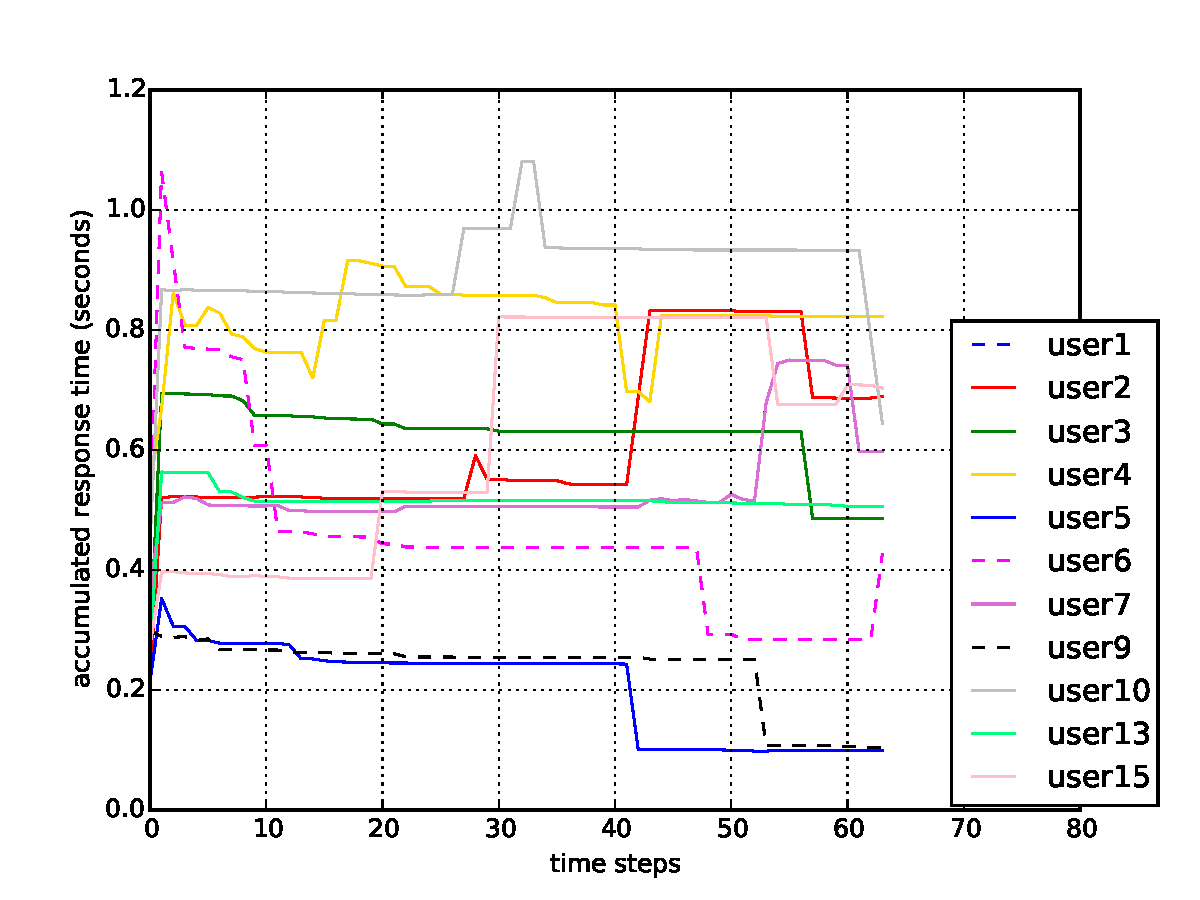
\includegraphics[width=\linewidth]{graphs/rt_step_lambda1}
\caption{ accumulated response time vs time step for several users extracted from the main data base for  $\bar{\lambda}_1 =[0.07075913789991828, 0.9292408621000817]$}
\end{figure}

\begin{figure}[h]
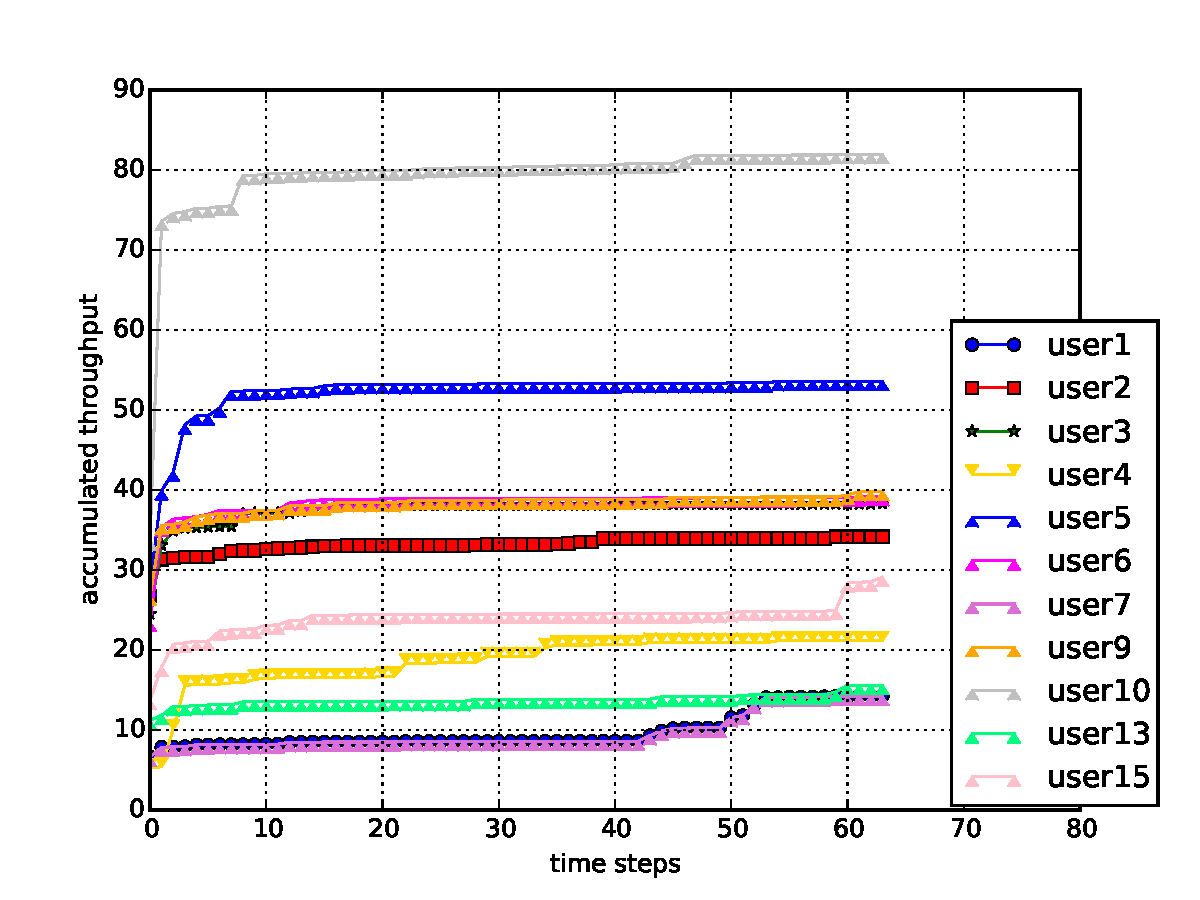
\includegraphics[width=\linewidth]{graphs/trough_step_lambda1}
\caption{accumulated throughout vs time step for several users extracted from the main data base for $\bar{\lambda}_1 =[0.07075913789991828, 0.9292408621000817]$}
\end{figure}

\begin{figure}[h] % Do not use only [h] in real documents.
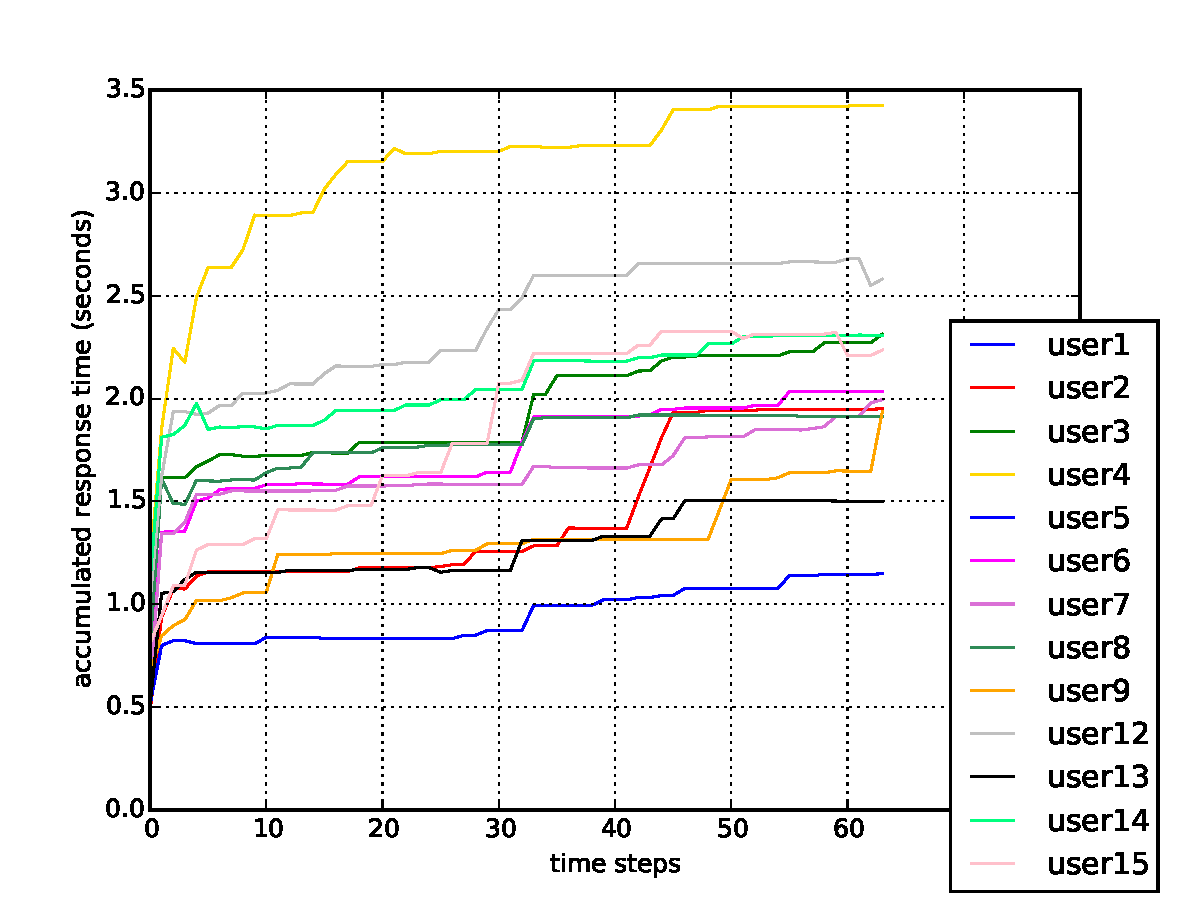
\includegraphics[width=\linewidth]{graphs/rt_step_lambda2}
\caption{ accumulated response time vs time step for several users extracted from the main data base for  $\bar{\lambda}_2 = [0.8573741847324399, 0.14262581526756013]$}
\end{figure}

\begin{figure}[h]
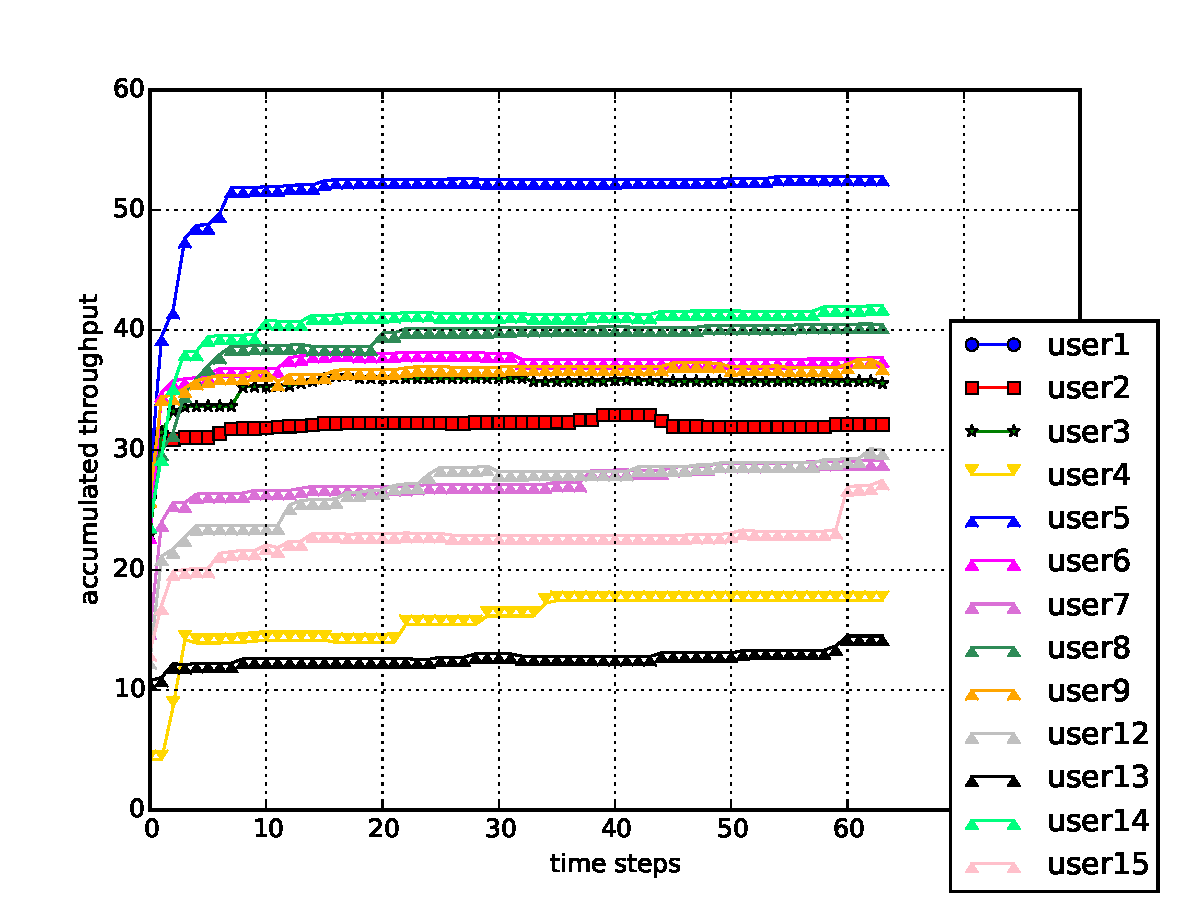
\includegraphics[width=\linewidth]{graphs/trough_step_lambda2}
\caption{accumulated throughout vs time step for several users extracted from the main data base for $\bar{\lambda}_2 = [0.8573741847324399, 0.14262581526756013]$}
\end{figure}

\begin{figure}[h] % Do not use only [h] in real documents.
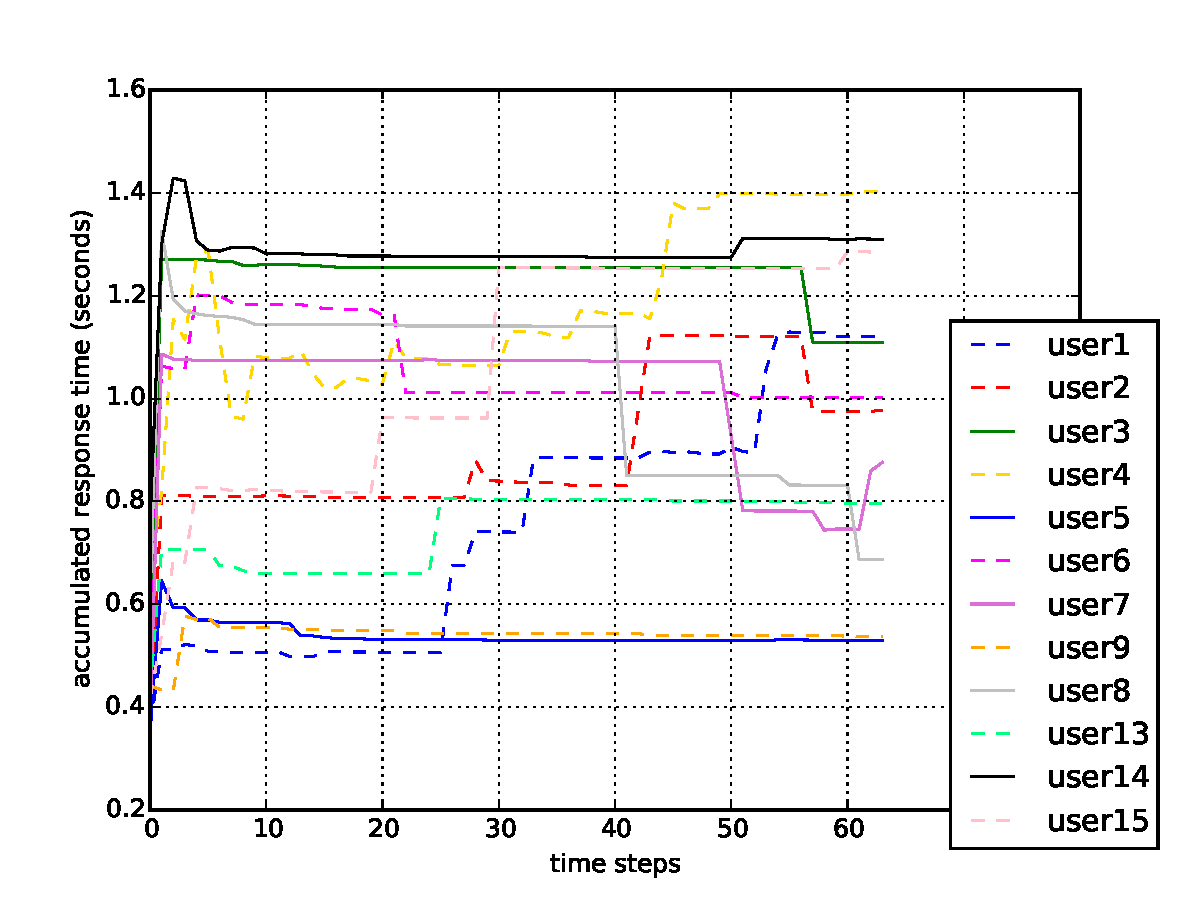
\includegraphics[width=\linewidth]{graphs/rt_step_lambda3}
\caption{ accumulated response time vs time step for several users extracted from the main data base for   $\bar{\lambda}_3 = [0.1696287781131175, 0.8303712218868825]$}
\end{figure}

\begin{figure}[h]
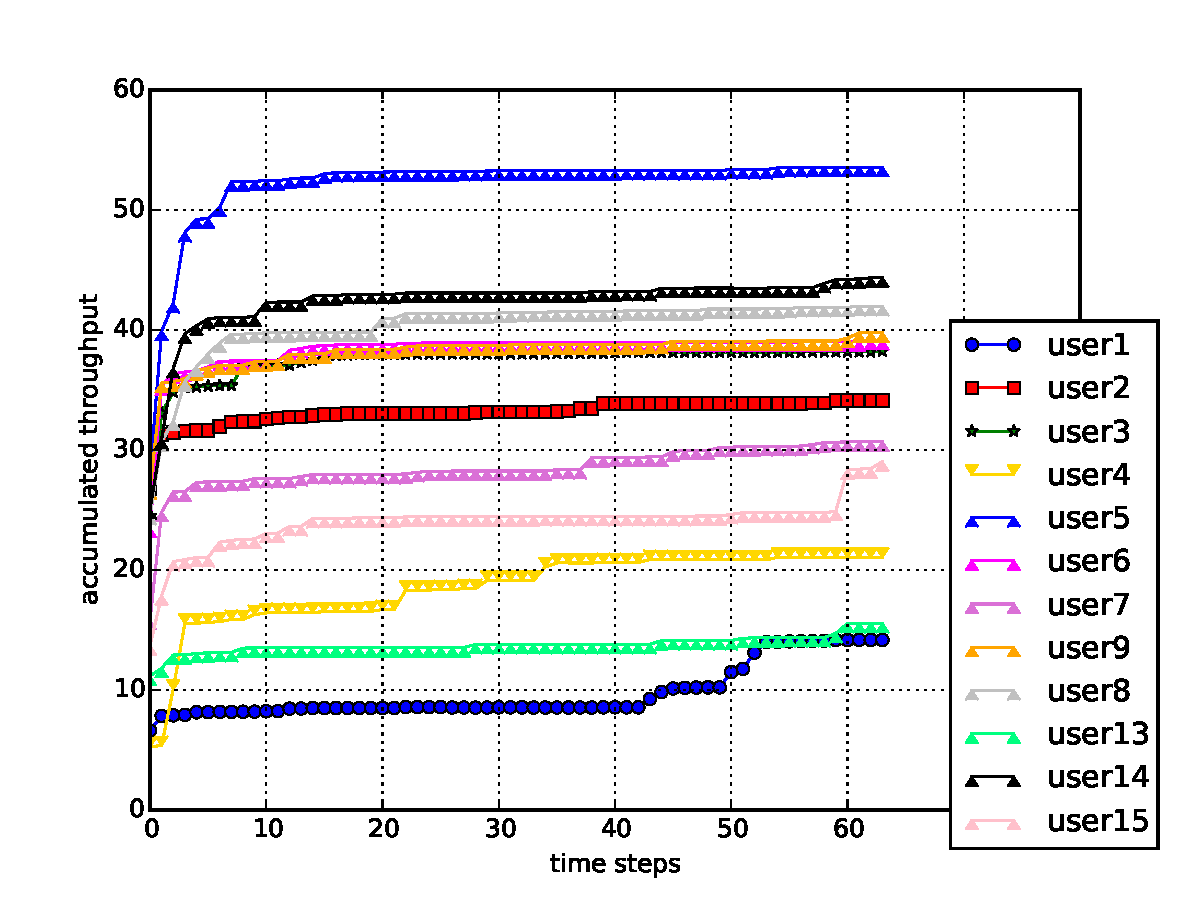
\includegraphics[width=\linewidth]{graphs/trough_step_lambda3}
\caption{accumulated throughout vs time step for several users extracted from the main data base for $\bar{\lambda}_3 = [0.1696287781131175, 0.8303712218868825]$}
\end{figure}

\end{document}